% %set_parent(‘/Users/mwilli/Documents/Spring_2017/Dissertation_Document/Dissertation_Working_Directory_Draft/Dissertation_Main.Rnw')
% 
% <<chunk_options, echo=FALSE>>=
% # This is where we set basic knitr options.
% opts_chunk$set(echo=TRUE, message=FALSE, warning = FALSE, cache = FALSE, comment="")
% options(width=75) # This sets how wide the R printout can be
% 
% 
%  <<setup-child, include=FALSE>>=
%  set_parent('/home/sam/Dissertation/Dissertation_Template/Dissertation_Main_Template/Dissertation_Main.Rnw')
% @
% 
% <<load_libraries, echo=FALSE>>=
% library(tidyr)
% library(dplyr)
% library(ggplot2)
% library(lme4)
% library(lsmeans)
% library(car)
% library(pbkrtest)
% library(xtable)
% library(cowplot)
% library(plyr)
% library(pander)
% library(memisc)
% @

\chapter{Human Speech Perception of Ear-Recorded speech\label{chapter3}}


\section{Introduction}\label{chap3:introduction}

This chapter introduces a human speech perception experiment in which humans' ability to accurately recognize ear-recorded and noisy mouth-recorded speech is compared.  In Chapter \ref{chapter2}, a data collection experiment was run to record speech recorded in both locations (at the mouth and in the ear) simultaneously.  The speech recorded from the ear was modified via pre-emphasis and low-pass filtering in order to make it more intelligible.  Further details about this study can be found in Section \ref{expt1} of Chapter \ref{chapter2}.

In order to judge the usefulness and intelligibility of the modified sounds recorded at the ear, it was necessary to run a human perception task using these recordings as stimuli.  Of primary interest to this task was whether the speech recorded at the ear in a noisy condition (a) had resulted in a sufficient reduction in the ambient noise level, and (b) was markedly more intelligible that speech recorded at the \textit{mouth} in a noisy condition.

\section{Background}\label{chap3:background}

% I need to demonstrate:
%   - Explaining the acoustic structure of speech in noise
%   - Demonstrating why speech in noise is difficult for humans to understand (mechanically? neurologically?)
%   - Explain the average/expected performance of Humans when recognizing speech in noise
%   - Show the variability in ability to understand speech in noise by different speakers.
Human listeners' inability to understand a speech utterance can occur from an information loss that might be caused by any of a host of factors.  For example, information can be lost in the domain of time (eg. an intermittent signal), from loss of intensity (eg. due to distance from the source), as well as the from distortion of the source itself, such as a speech impediment (\cite{mattys:12}).  Of particular interest to the present study is the difficulty for human listeners to understand a speech signal due to excessive, additive background noise from sources other than the desired speech signal.

The ability of the human auditory system to hear and differentiate multiple sources of sound from a single pressure wave is often given the term `auditory scene analysis' (\cite{bregman:94}).  The term `scene analysis' was borrowed from the visual domain, implying the separation of a `scene' (be it auditory or visual) into its component objects (again, be they auditory or visual). For the purposes of this study, this background discusses the human auditory ability to find multiple sound sources from a temporal stream of air pressure fluctuations (ie. sound) reaching the tympanic membrane.

To visualize the auditory scene, note the waveform (ie. the graph of air pressure fluctuations) that reaches the tympanic membrane in Figure \ref{fig:animal_singlechannel}.  
%
\begin{wrapfigure}{r!}{0.5\textwidth}
\centering
  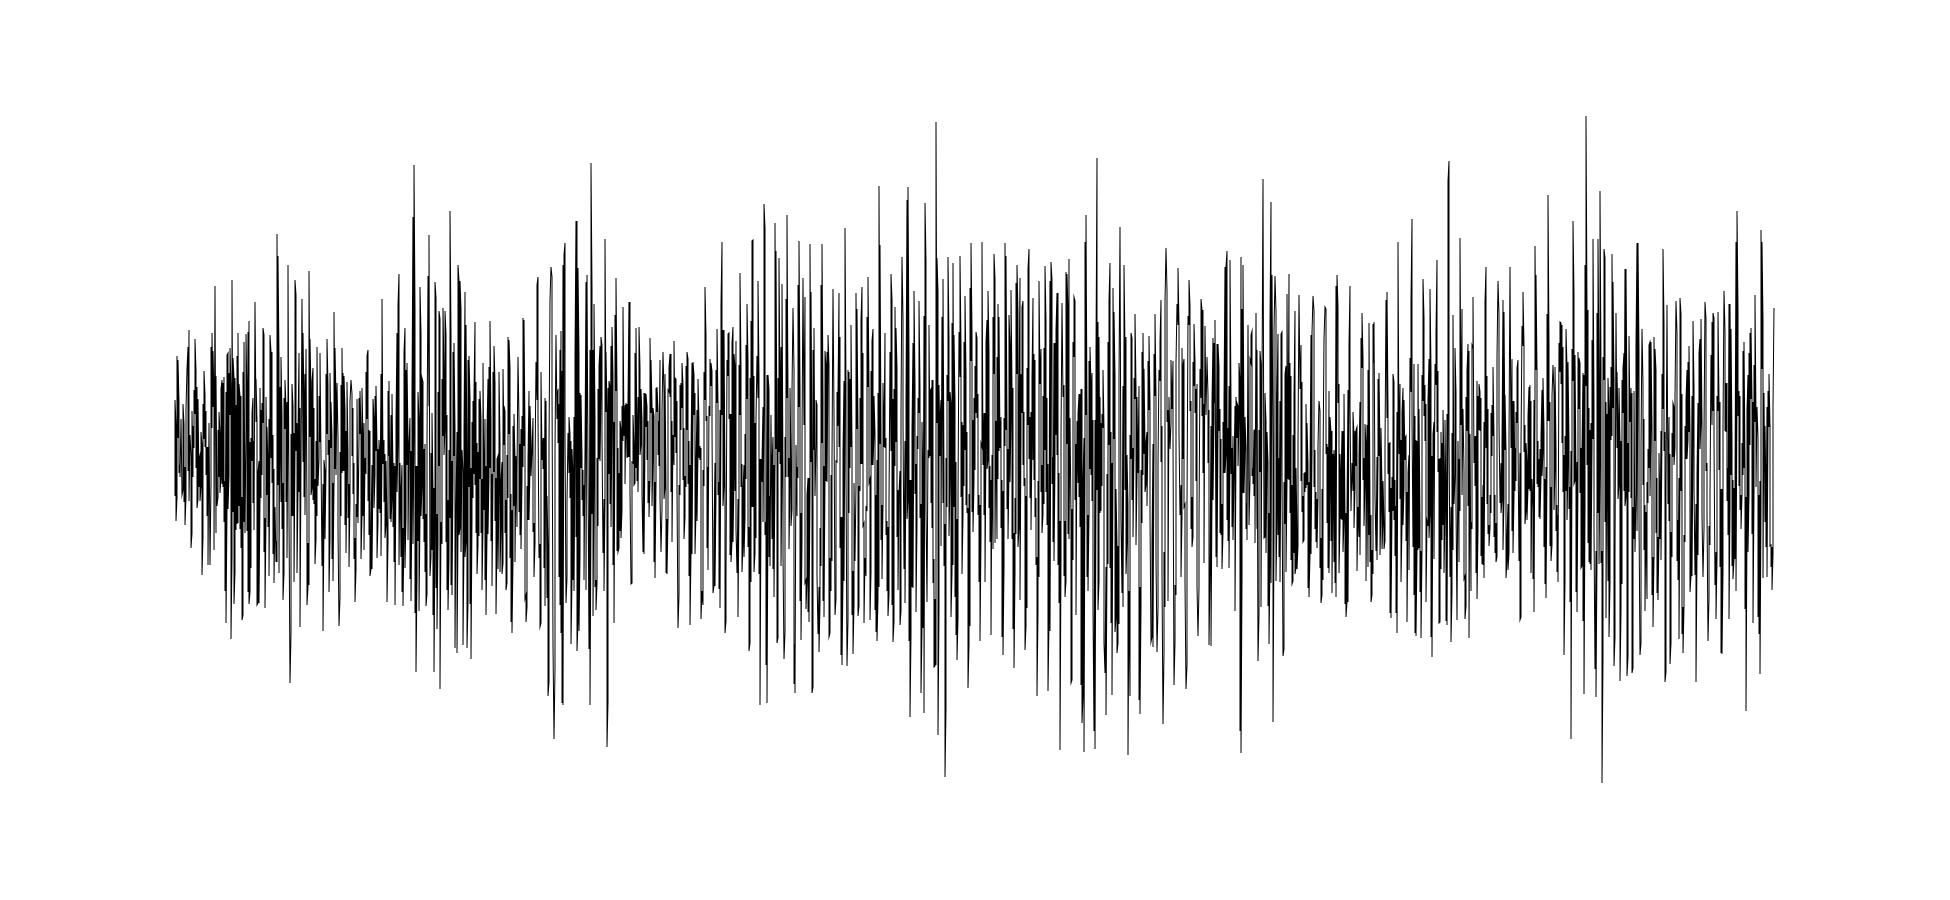
\includegraphics[width=0.45\textwidth]{figure/single-channel-animals.png}
  \caption{A waveform composed of multiple sound sources (cf. Fig. \ref{fig:animal_multichannel}).}
  \label{fig:animal_singlechannel}
\end{wrapfigure}
%
It is composed of all environmental sounds contributing to the air pressure fluctuation at the tympanic membrane\footnote{Note that this is for illustration purposes; the waveform will obviously look different when shaped by a given environment and the human ear canal before reaching the tympanic membrane.}.

However, using the framework of auditory scene analysis, the human auditory system is able to separate this input signal into its various sources, or `auditory objects'.  The auditory system separates the above waveform into its actual component sources of human speech, and the sounds of a sheep, cow, and horse, seen in Figure \ref{fig:animal_multichannel}; ``The normal auditory system exhibits a remarkable ability to parse these complex scenes'' (\cite{middlebrooks:17}, 2).

Of course, there reaches a point at which the auditory system fails and can
%
\begin{figure}[h!]
\centering
  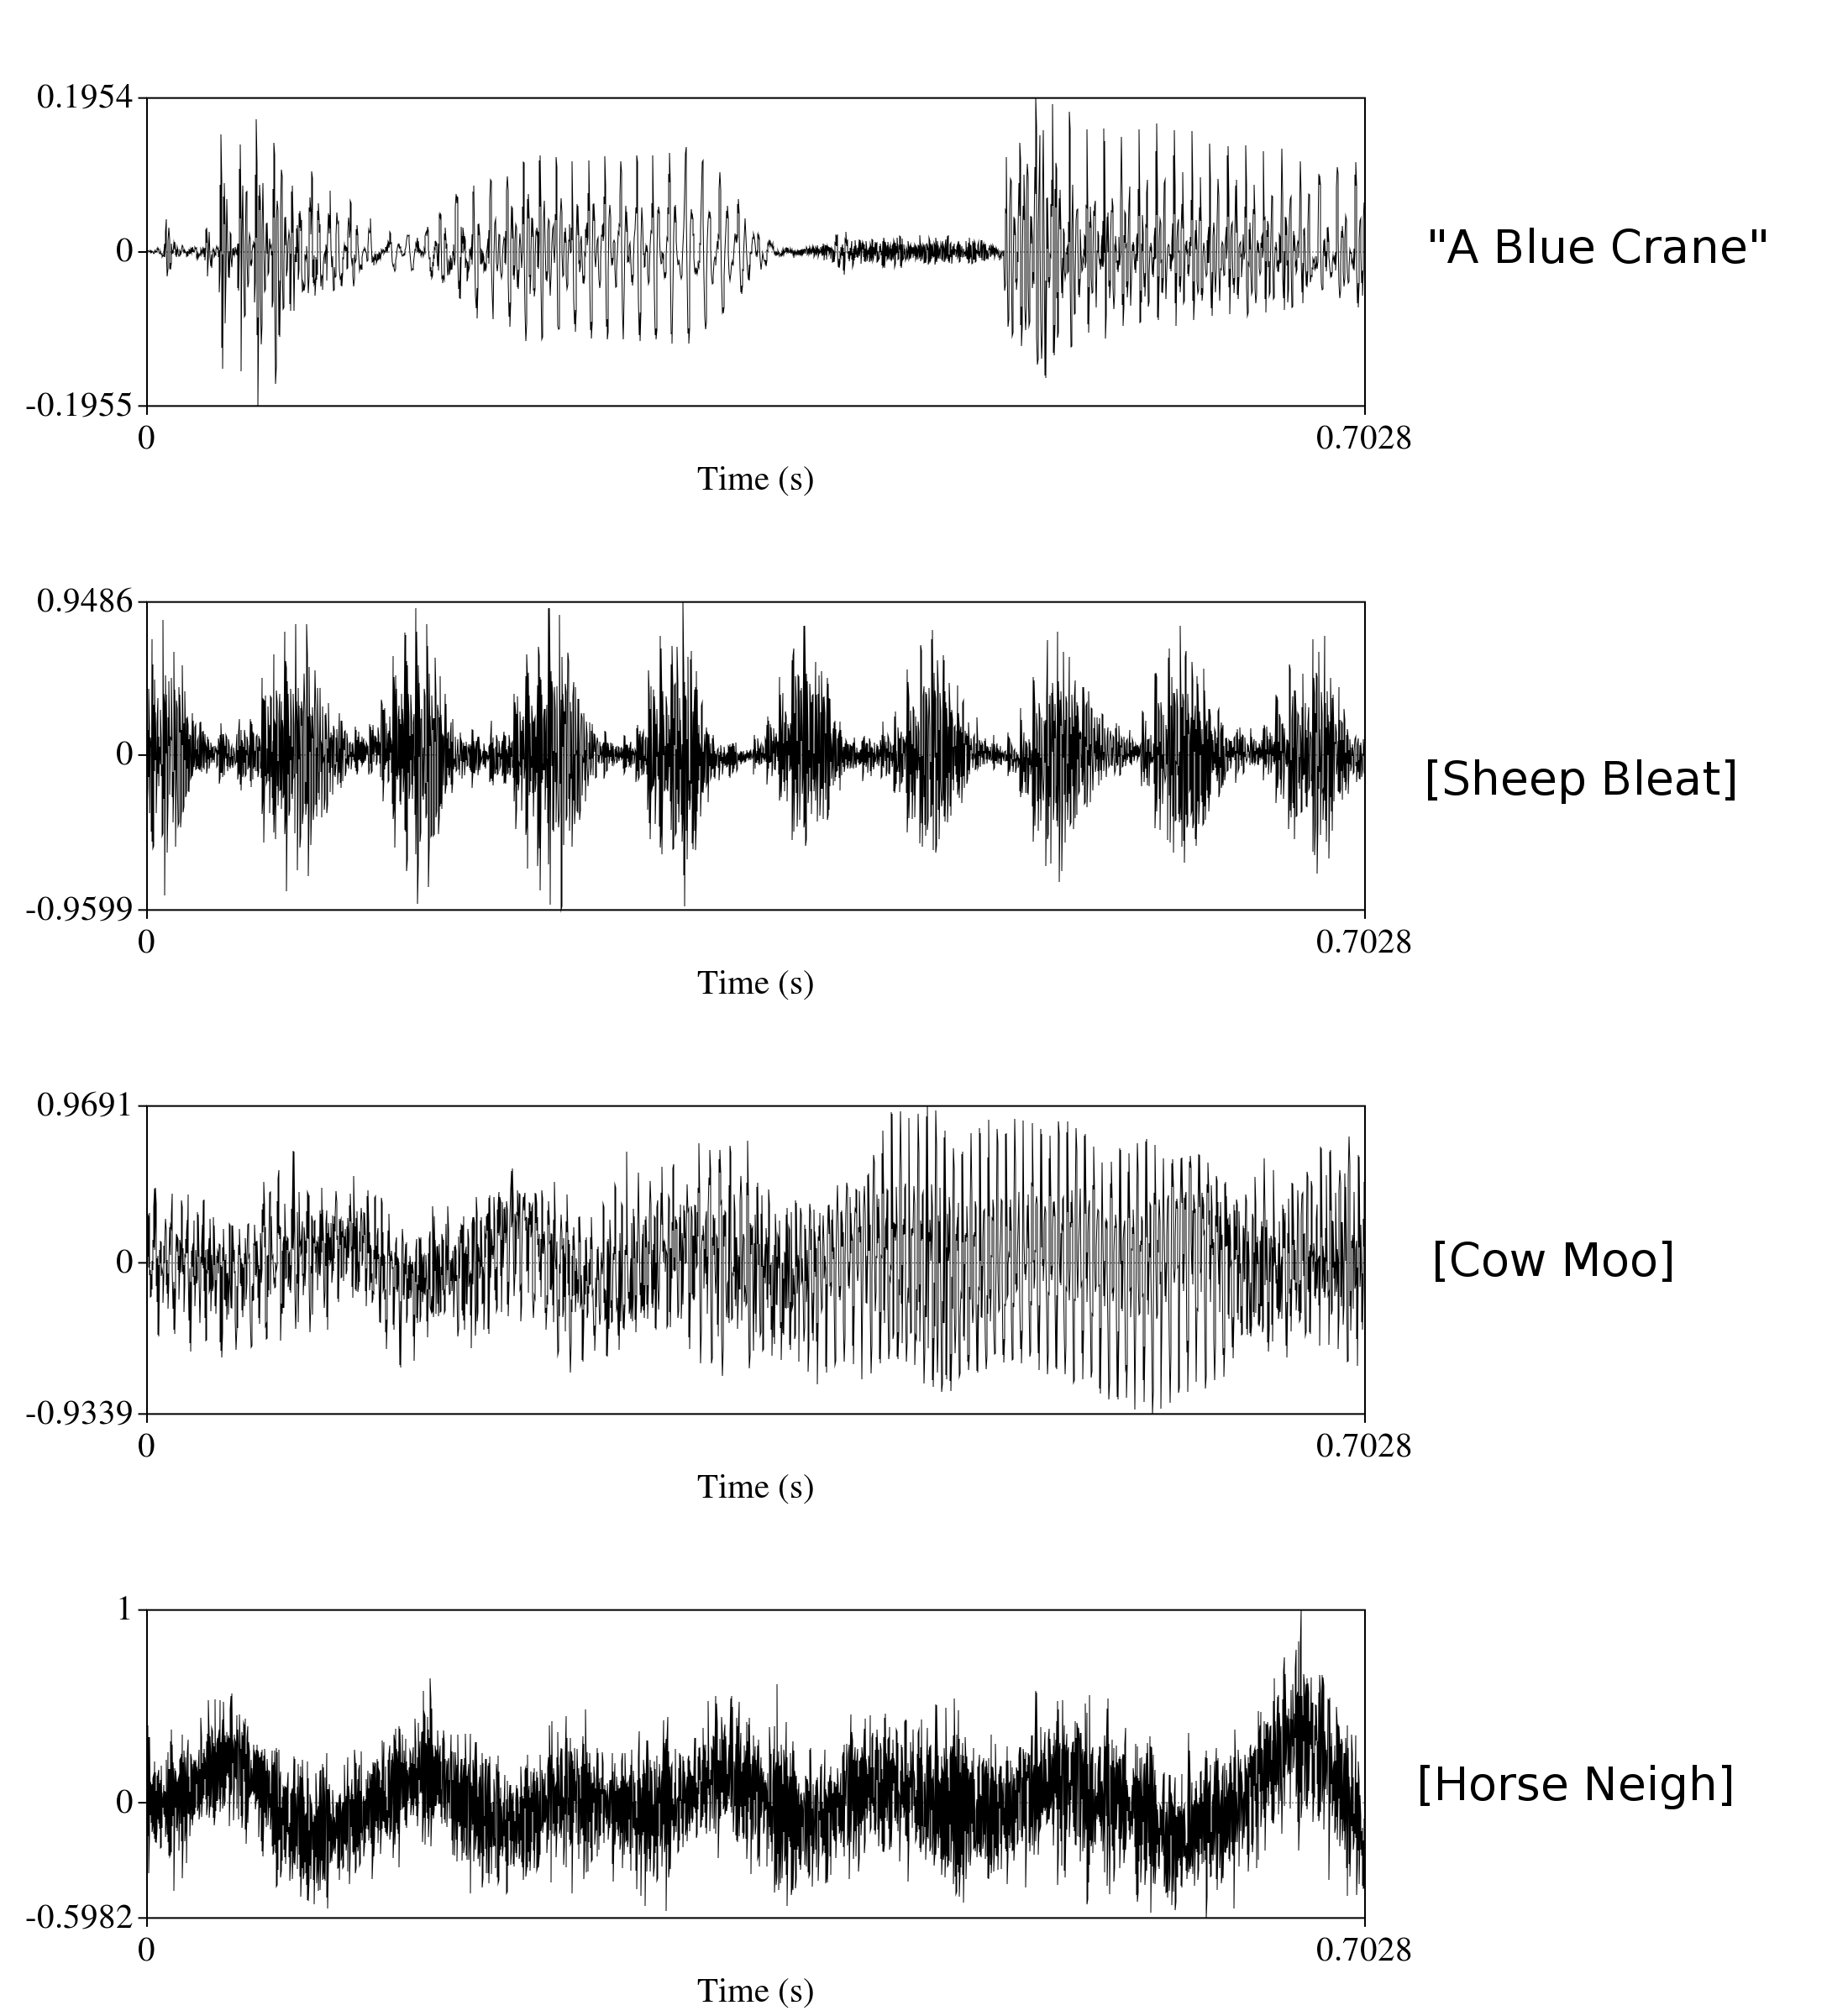
\includegraphics[width=0.95\textwidth]{figure/animal_multichannel-w-text.png}
  \caption{The four component waveforms (human speech, sheep, cow, horse), of the combined waveform seen in Figure \ref{fig:animal_singlechannel}.}
  \label{fig:animal_multichannel}
\end{figure}
%
 no longer differentiate all sources. Pertaining to the present research, there reaches a point at which the auditory system cannot recognize the information in a human speech signal when embedded with background noise from one or more additional sources.  The following section reviews the acoustics of speech in noise in more depth .
  
\subsection{Acoustics of Speech in Noise}
\label{bkgrnd:speech_in_noise}

Speech in noise can be intuitively grouped into two components, the speech (more specifically the voice one is intending to hear) and the noise, called the `masking' element.  Broadly, masking is defined as ``the process by which the threshold of hearing for one sound is raised by the presence of another'' (\cite{ansi:13}, 61).  This masking element is everything \textit{but} the voice\footnote{For the purposes of this paper, the term `voice' will be used throughout to refer to the singular speech source the listener desires to hear out of the masked signal.} (speech signal) that one is interested in, as it was intended to be heard.
%which, as indicated in Chapter \ref{chapter2}, could be of any form or loudness.

The masking process can be broken down into two forms: energetic masking and informational masking.  Energetic masking occurs when the masking element shares the same temporal and frequency elements of the voice.  In a sense, the masked element and the voice `compete' for `space' along the basilar membrane and then the auditory nerve (\cite{brungart:01}), but they also compete for the listener's attention (ie. the listener must concentrate on ignoring the mask, and exclusively listening to the target, (\cite{mattys:12})).  Energetic masking is normally thought to occur primarily in the `lower auditory processes, eg. the cochlea and auditory nerve, though this is not always the case, as described further below.  

Informational masking can be broadly thought of as difficulties relating to memory, linguistic processing, and the like, oftentimes generalized to speech-on-speech noise.  \cite{mattys:10} failed to find informational masking in a cross-linguistic task, and so it is possible that informational masking could be limited to situations in which the masking speech is intelligible. This type of masking is thought to occur primarily in the `higher auditory processes' in the brain.

An instance of both energetic and informational masking can be visualized in a diagram of overlapping speech presented in \cite{middlebrooks:17}, and seen in Figure \ref{fig:sos-masked-spctgrms}.
%
\begin{figure}[h!]
\centering
  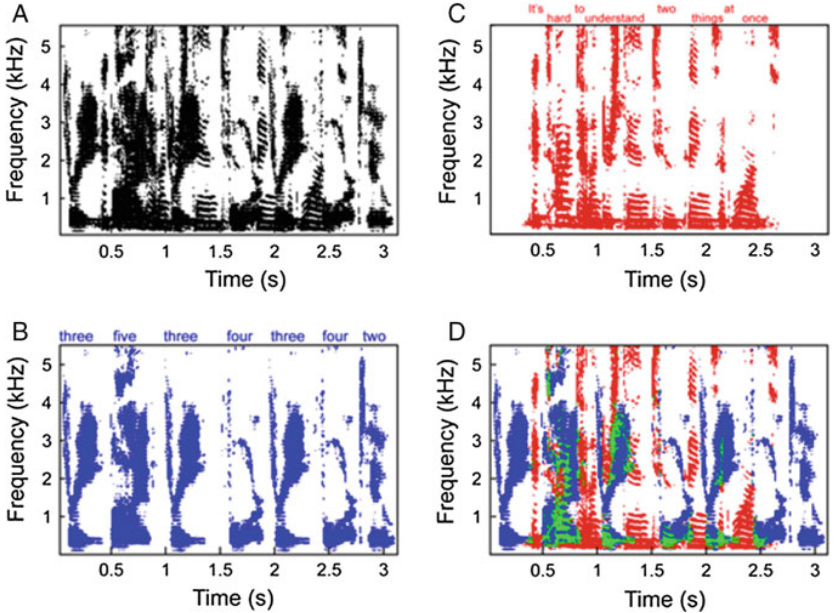
\includegraphics[width=0.95\textwidth]{figure/speech-on-speech_masked_spectrograms.png}
  \caption{Diagrams of different spectograms. (A) The spectogram of two temporally overlapping spoken utterances. (B) The spectogram of the utterance ``three five three four three four two'' colored in blue (C) The spectogram of the sentence ``It's hard to understand two things at once.'' colored in red. (D) The overlap of the two spectograms (B) and (C), with the color green highlighting the areas of energy in frequency and time that overlap. }
  \label{fig:sos-masked-spctgrms}
\end{figure}
%
Utterance (C) in the figure is the desired `voice', leaving utterance (B) the masking element.  In (D), one can see the voice (red), the areas of masking in which there is direct frequency and temporal overlap (green), and the remainder of the masking speech (blue). Of course this is never so nicely differentiated, and the resulting acoustic information that the auditory system receives can be seen in (A), in which no source is differentiated.  This is primarily a form of energetic masking (competition for lower-level processing), though upper level processing is required to take meaning from the desired voice, which is masked informationally by the competing voice with its own information.

The five different background noises used in the study described in Chapter \ref{chapter2} (data collection of speech recorded at the ear) energetically mask the voice in the signal.  A small (5 second) portion of the spectrogram of each sound can be seen in Figure \ref{fig:bkgrnd-noises}.  These sounds don not produce any competing linguistic informational content themselves which mask the desired voice (the `caf\'{e}' noise, seen in Figure \ref{fig:cafe-bkgrnd}, does contain speech babble, none of it intelligible), and so masking occurs by producing energy at the same time as - and in the same frequency range as - the recorded voice.

\begin{figure}[h!]
\begin{subfigure}{0.475\linewidth}
  \centering
  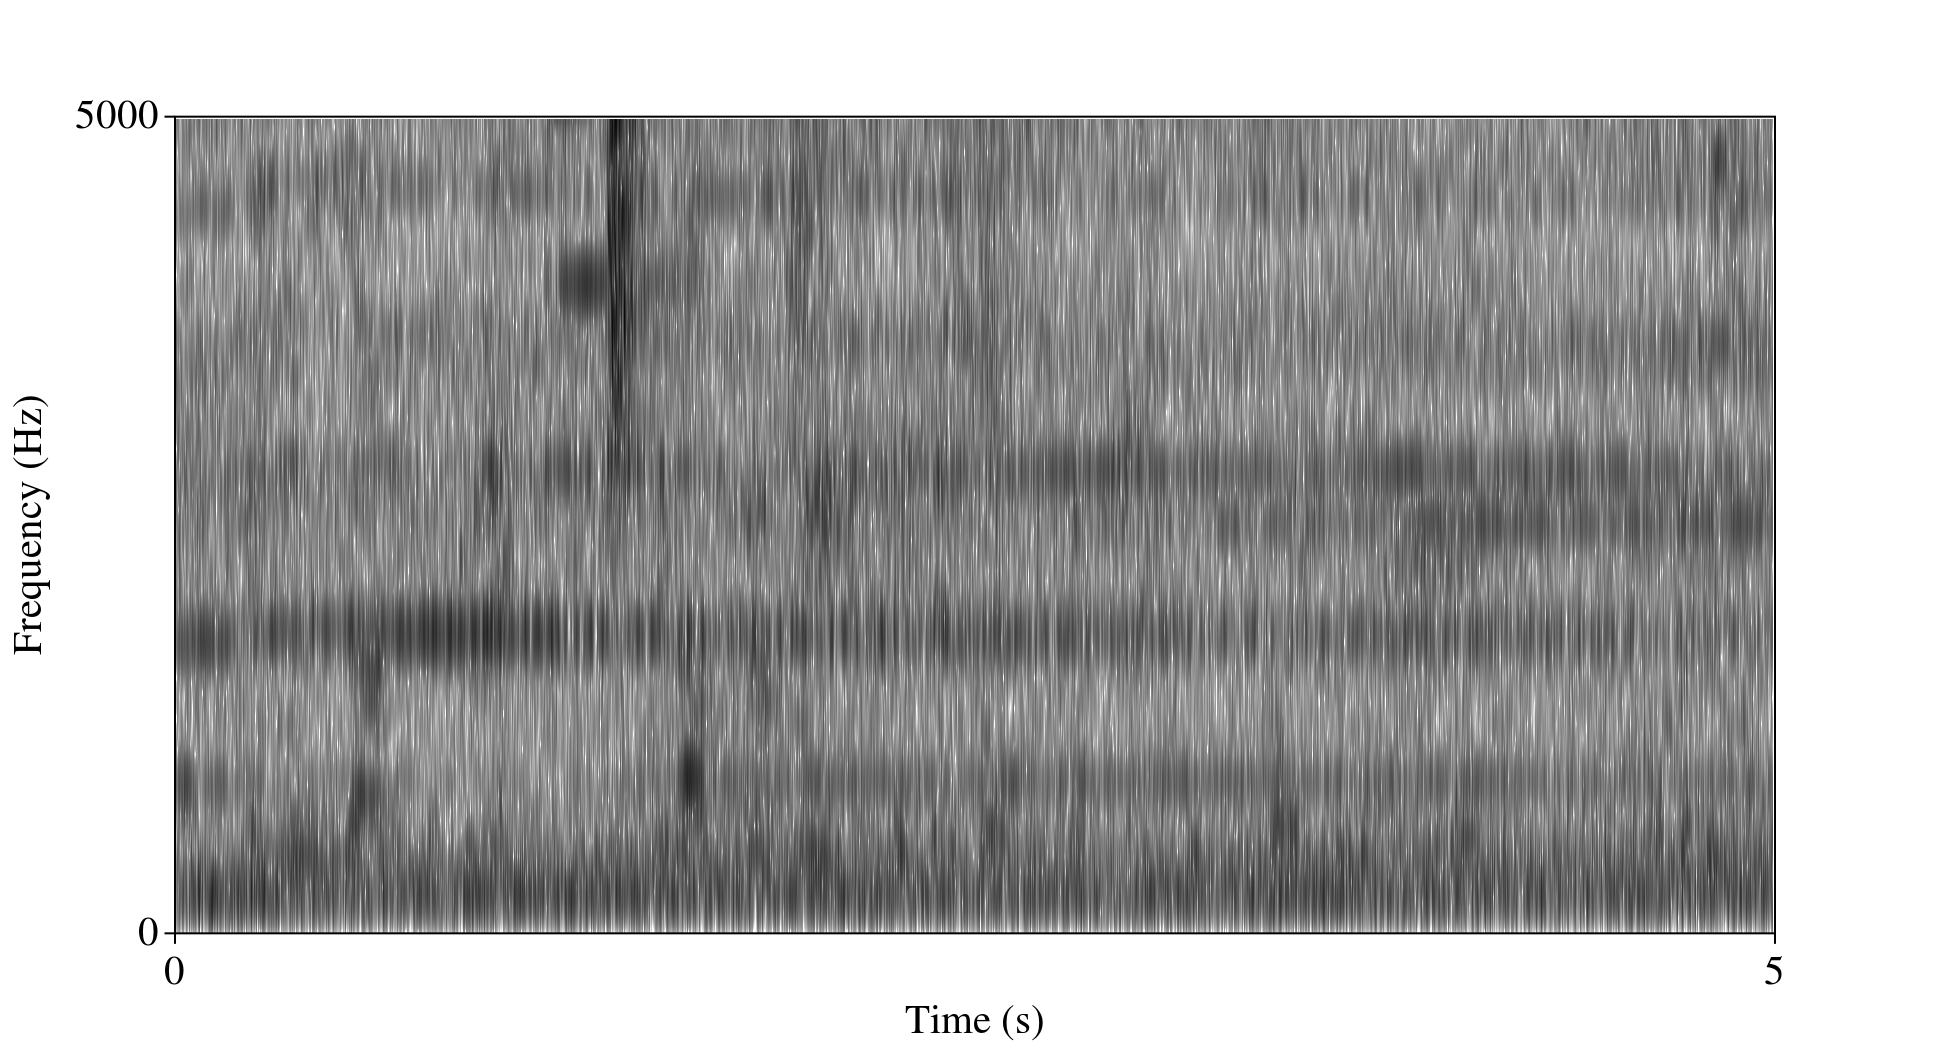
\includegraphics[width=0.9\textwidth]{figure/spctgrm-bus-background.png}
  \caption{Bus background noise.}
  \label{fig:bus-bkgrnd}
\end{subfigure}
\qquad
\begin{subfigure}{0.475\linewidth}
  \centering
  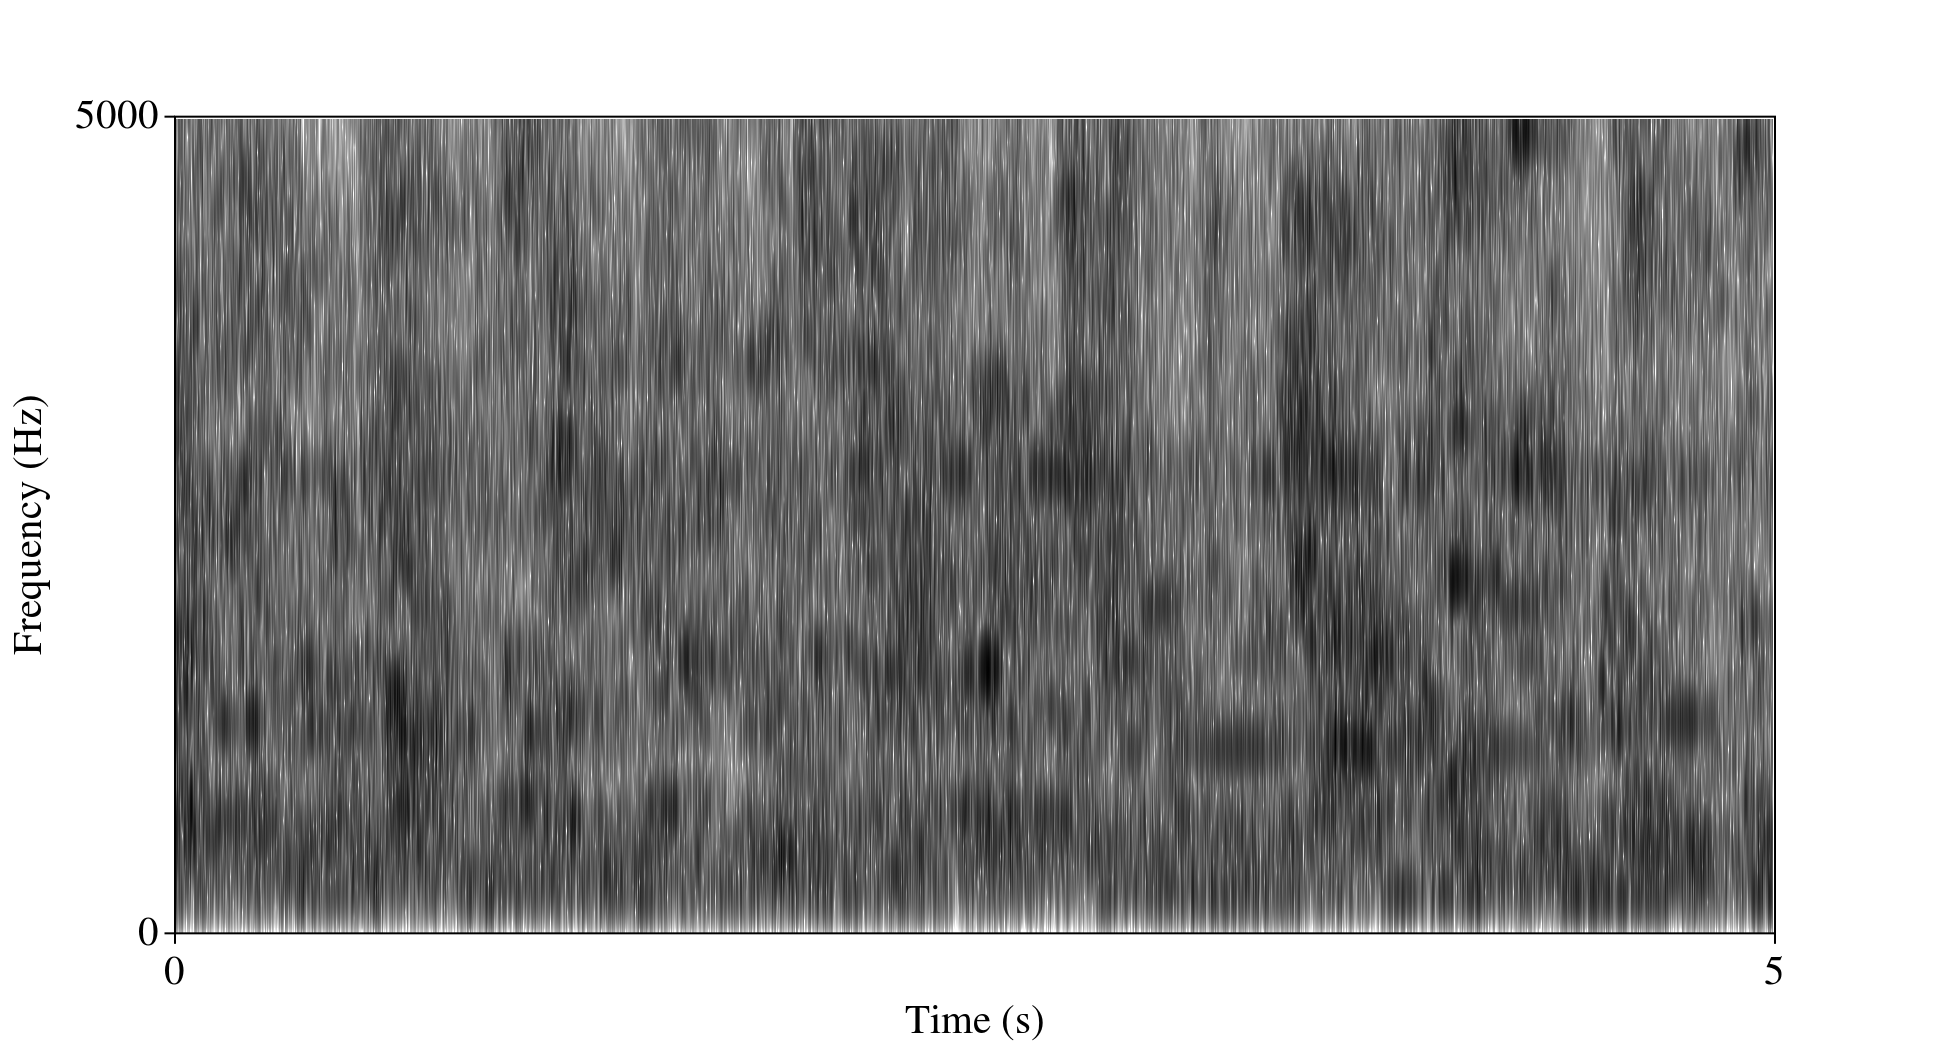
\includegraphics[width=0.9\textwidth]{figure/spctgrm-cafe-background.png}
  \caption{Caf\'{e} background noise.}
  \label{fig:cafe-bkgrnd}
\end{subfigure}%
%\hfill
\\[2ex]
\begin{subfigure}{0.475\linewidth}
  \centering
  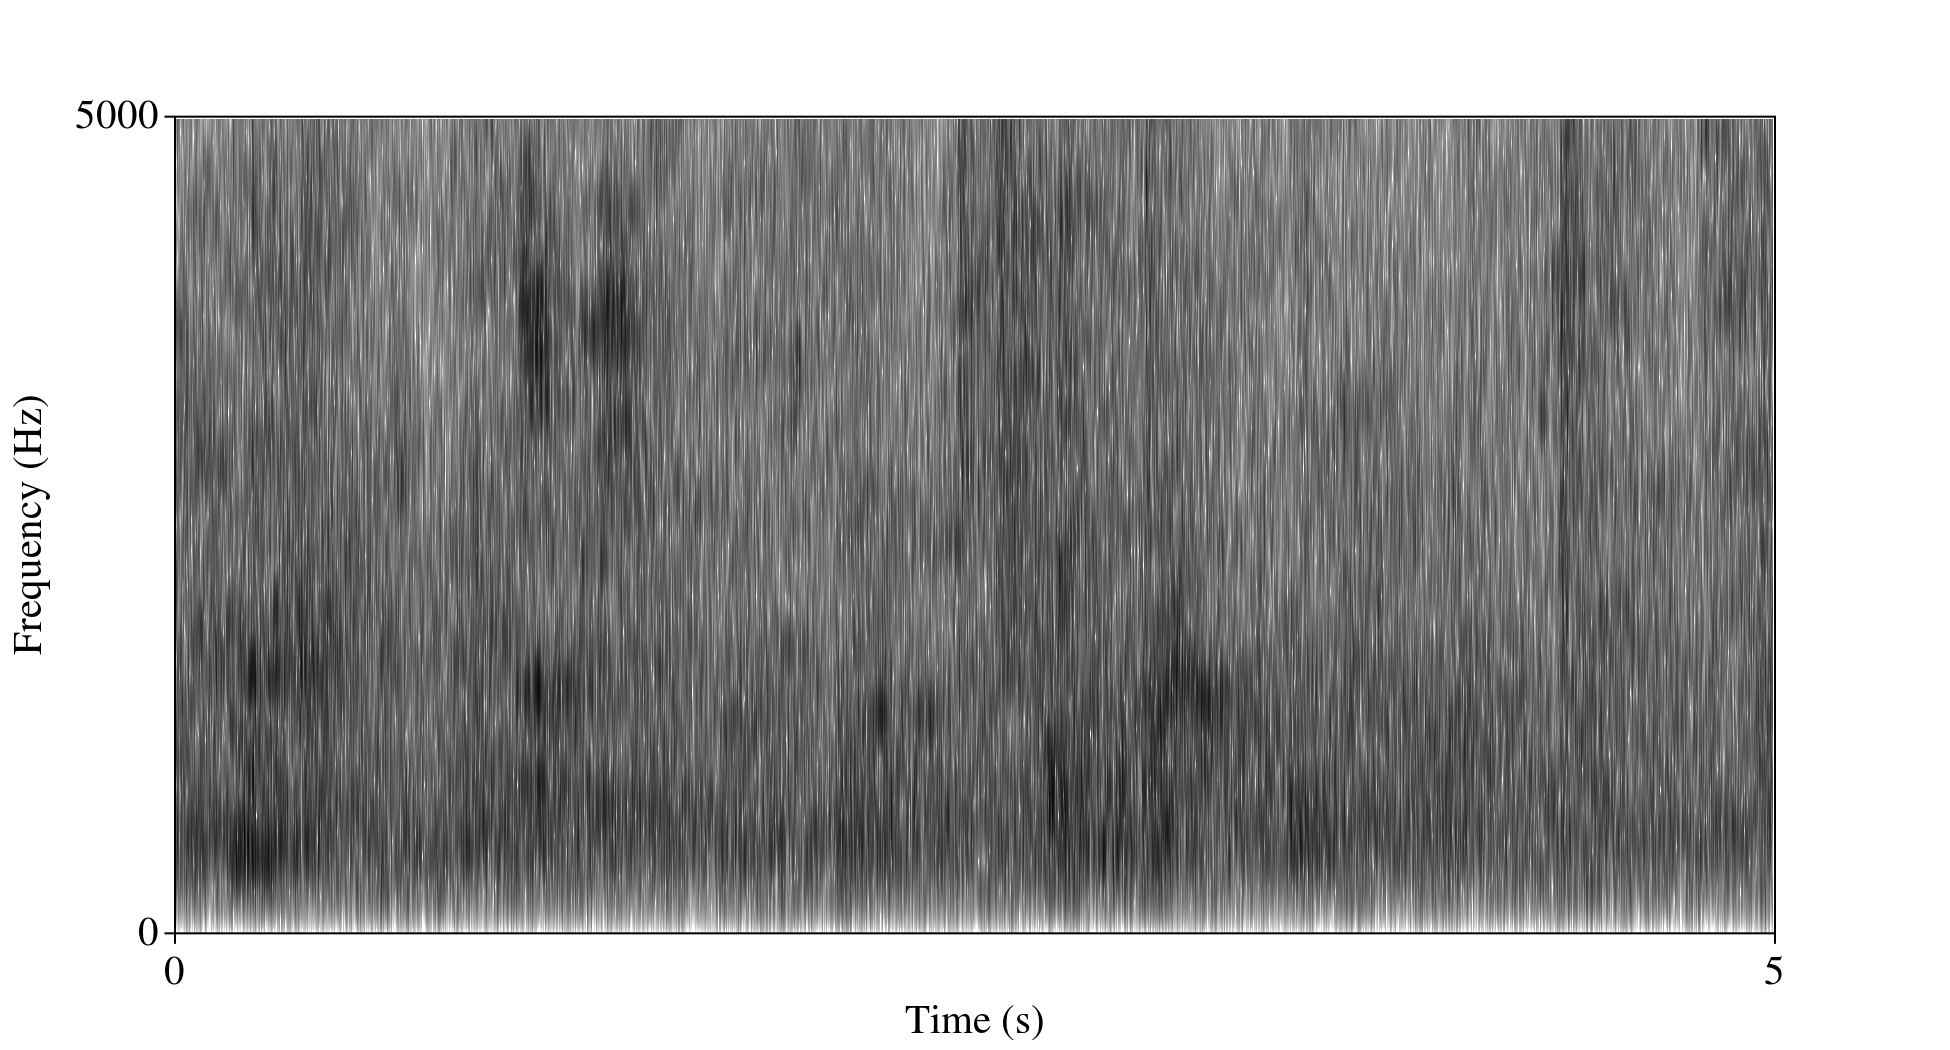
\includegraphics[width=0.9\textwidth]{figure/spctgrm-ped-background.png}
  \caption{Pedestrian background noise.}
  \label{fig:ped-bkgrnd}
\end{subfigure}
\qquad
\begin{subfigure}{0.475\linewidth}
  \centering
  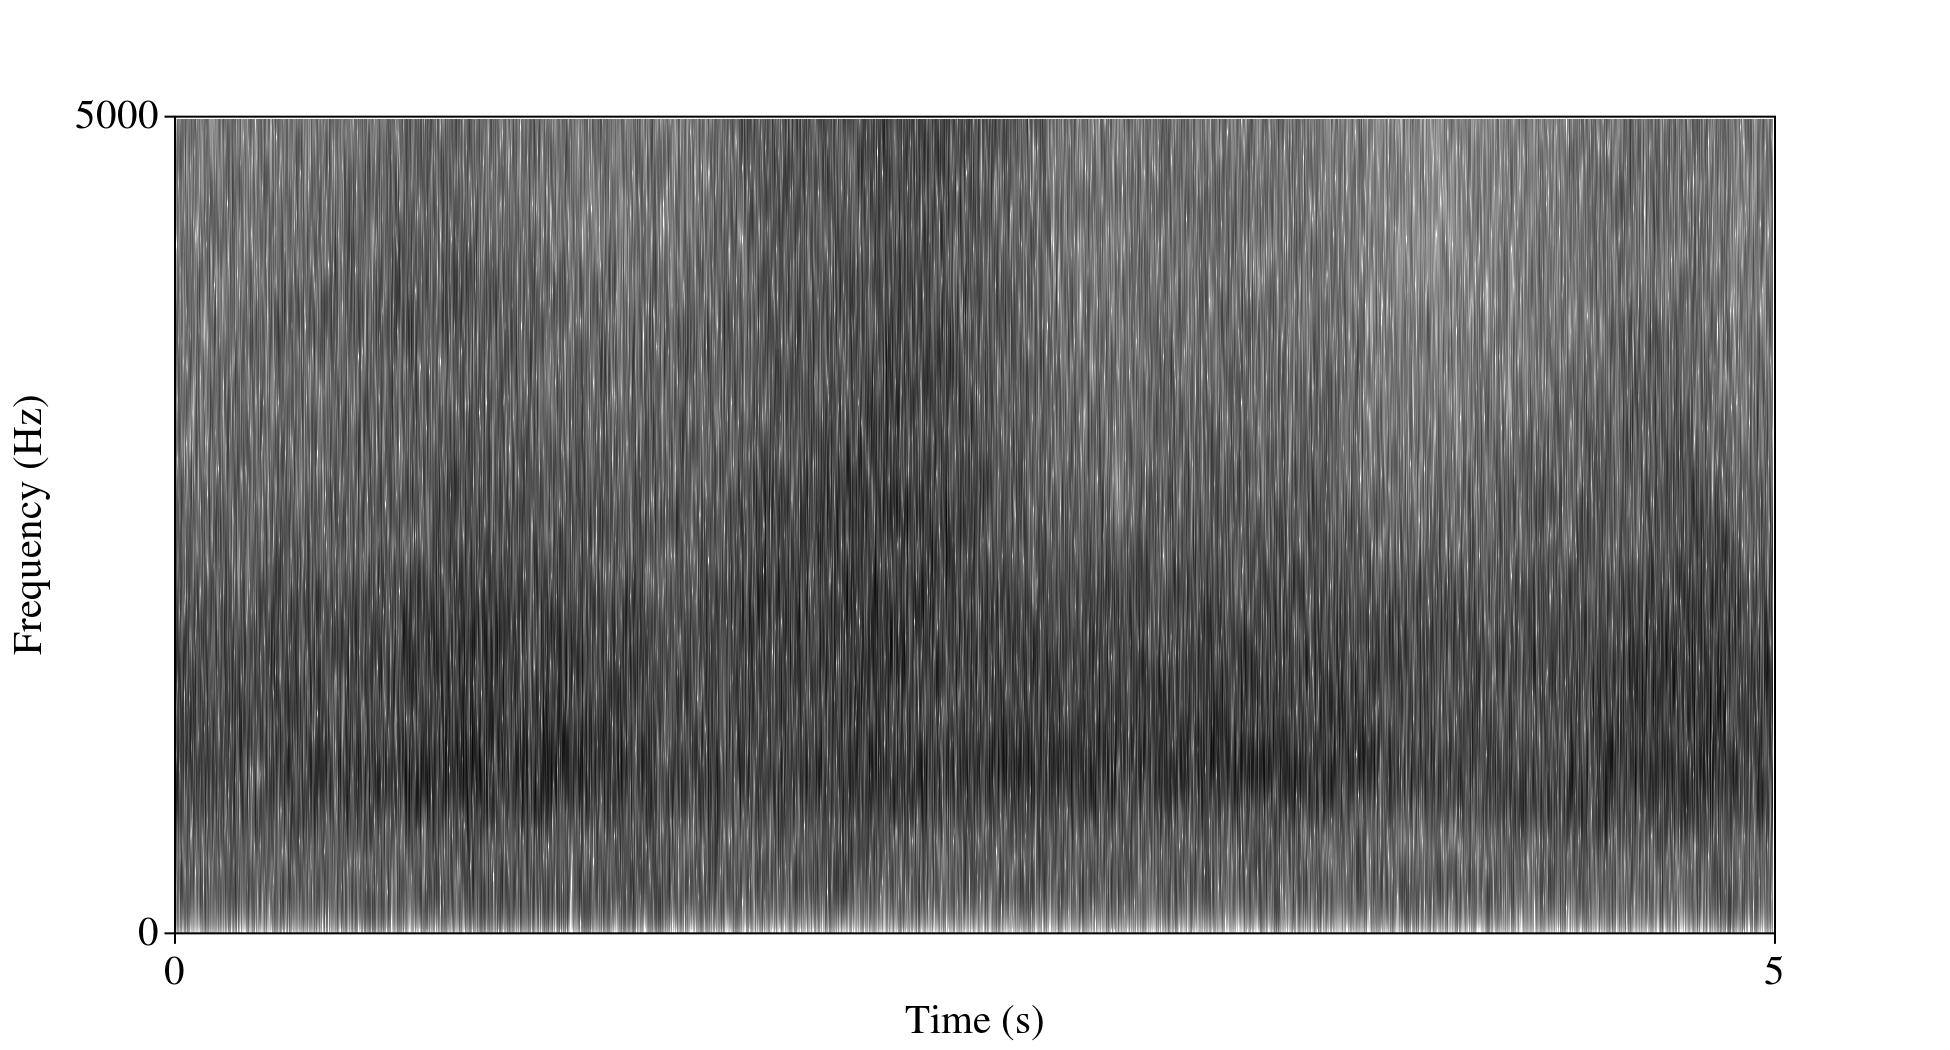
\includegraphics[width=0.9\textwidth]{figure/spctgrm-str-background.png}
  \caption{Street background noise.}
  \label{fig:str-bkgrnd}
\end{subfigure}%
%\hfill
\\[2ex]
\begin{center}
\begin{subfigure}{0.475\linewidth}
  \centering
  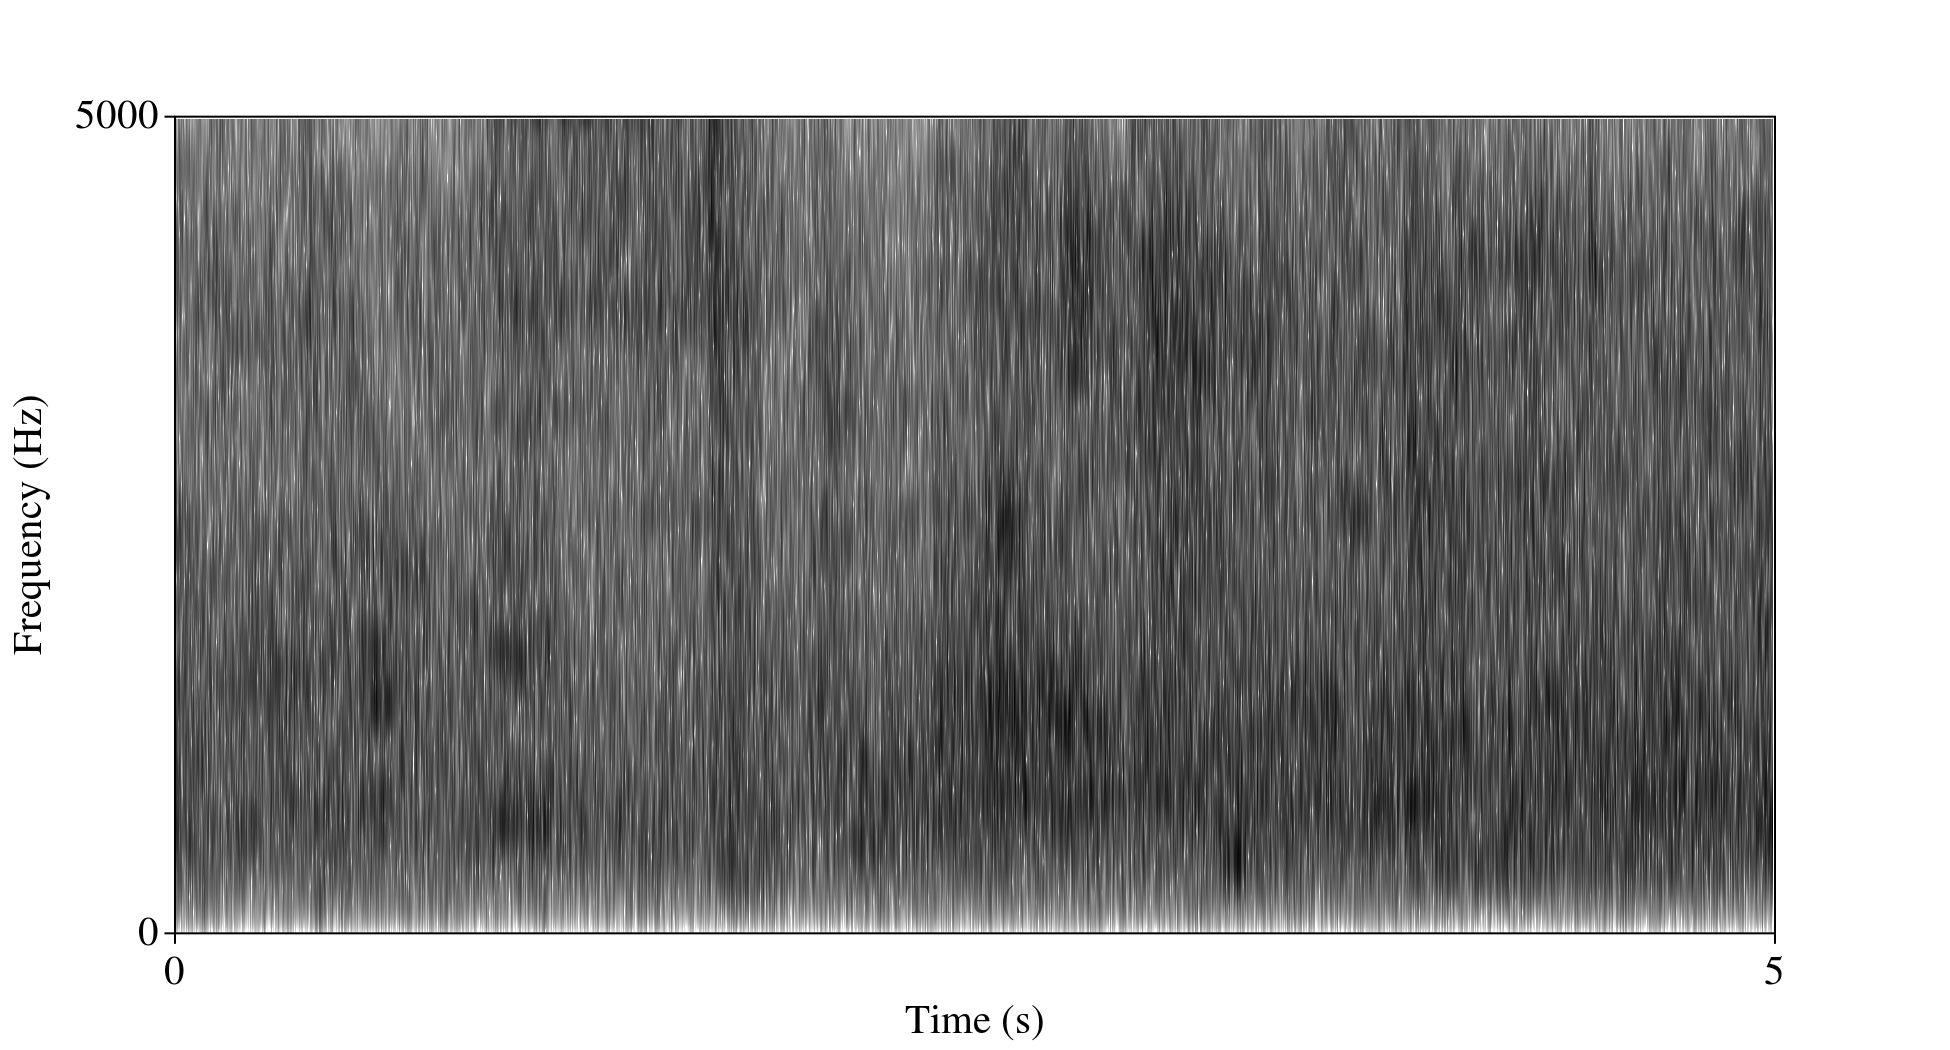
\includegraphics[width=0.9\textwidth]{figure/spctgrm-fac-background.png}
  \caption{Factory background noise.}
  \label{fig:fac-bkgrnd}
\end{subfigure}
\end{center}
\caption{Example spectograms of the first five seconds of the background noise tracks. Most recorded sentences occurred within these temporal spans.}
\label{fig:bkgrnd-noises}
\end{figure}

Simply because a voice may be `masked' by noise does not necessarily mean that the voice is not heard or understood.  The auditory system employs a number of methods to overcome the masking and interpret the voice; this process is termed the `release from masking' (\cite{middlebrooks:17}).  One such theorized method - the use of humans' built-in binaural hearing - uses both ears to tease apart the different sources, exploiting the very small temporal difference that occurs when different sound sources reach each ear.  
In the example of binaural hearing, it is easy to see that energetic and informational masking are not strictly limited to separate `lower' and `higher' processes, respectively (\cite{durlach:06}).
Binaural hearing is an example of a `higher' process `releasing' energetic masking, as it necessarily requires signals from both ears (ie. the joining of the signals from both auditory nerves) to be used (\cite{hirsh:48}). It makes use of the spatial directionality of the noise(s) from the listener to separate the different sources (\cite{bregman:94}).

There are many other methods theorized to be a part of the auditory system's ability to release energetic masking.  One involves making note of acoustic transitions: ``when [a] sound...changes its properties gradually, [it] is likely to be heard as a single changing sound.  However, when [it] changes...abruptly, [it] tends to be treated as a newly arriving sound, this tendency increasing with the abruptness of the change.'' (\cite{bregman:94}, 5).  The use of fundamental frequency (F0) has also been shown to be an effective tool, presumably to interpret the location of harmonics, and parse apart different sources (eg. two separate, simultaneous vowels with different F0s, (\cite{bird:97})). %Other methods, particularly among informational masking (\cite{middlebrooks:17}), are beyond the scope of this project.

\cite{mattys:12} briefly discussed the concept of `training' in the sense that one can learn to accommodate a particular adverse condition (eg. background noise, signal distortion, etc.) with practice in that area.  This, in theory, allows a listener to identify which methods of release from masking are most effective, and to practice the use of these methods within the specific adverse condition.  Learning is less effective in cases which the degradation is variable or unpredictable between trials, such as with unpredictable background noise.


\subsection{Performance of Human Recognition of Speech in Noise}

Eventually, with enough background noise and masking, the methods listed above for releasing the masking fail and recognition begins to break down.  Under the most simple conditions to measure - steady-state noise - \cite{ding:13} reported that when listening to speech in noise, human self-reported intelligibility ratings did not drop significantly until the SNR reached approximately -3 dB, where intelligibility dropped to about 55\%;  it did not reach 0\% self-reported intelligibility until the signal had -9 dB SNR.

This subjective measure was backed by a study performed by \cite{gilbert:13}, who used the PRESTO corpus (\cite{garofolo:93}) to test sentence intelligibility among 121 native English speakers.  \cite{gilbert:13} found that - similar to \cite{ding:13} - the median score (at the 50th percentile) of speech with a -3dB SNR had about 55\% accuracy.  At +3 dB SNR, the median score increased to approximately 88\% accuracy.

\cite{ding:13} mentioned that there was great inter-speaker variation among the self-reported, subjective perception of intelligibility of an utterance; this was also supported by \cite{gilbert:13}'s results. The latter showed that, averaging over all SNR conditions (-5, -3, 0, +3 dB), the variability between speaker's accuracy scores had a range of almost 36\% for a given item.  A retest performed with a subgroup of the original participants on the same dataset yielded a similar (~34\%) range of variability in accuracy.  

\cite{francis:10} discussed how listening to speech in background noise places extra demands on working memory, as does listening to degraded speech (\cite{francis:09}).  The diversion of working memory to acoustic processing can be particularly detrimental to performance when a listener simultaneously works on other computation, eg. syntactic and semantic parsing (eg. phrase or sentence recognition \cite{caplan:99}). \cite{tamati:13} tested a group of high-performing hearers of speech in noise against a separate group of low-performing hearers (all had `normal' hearing) using several different working- and short-term memory tasks.  Not surprisingly, the group of listeners who are able to better hear speech in noise also perform statistically better on the working memory tasks.  Working- and short-term memory are by no means the only indicators of perceptual performance.


\subsection{Summary}

Speech in noisy environments presents a challenge for recognition.  Competing acoustic energy from different sources blends together into a single signal that reaches the ear.  The energy from these sources occurs at the same temporal and frequency locations, and can `compete' for space along the auditory pathway.  Energetic masking largely refers to the direct masking of the acoustic energy of the desired voice.  Informational masking largely occurs when there are multiple, intelligible voices that compete for attention.

The auditory system employs many methods to release the desired voice from masking.  These include binaural hearing, the use of acoustic transitions, the use of pitch information, and many others.  Practice recognizing speech in a specific adverse condition allows a listener to improve their recognition accuracy when listening to that adverse condition in the future.  Despite these tools of the auditory system, it is often the case that the background noise is too loud for them to work effectively.  Studies by \cite{ding:13} and \cite{gilbert:13} indicated the range of SNRs in which human speech perception begins to falter substantially.

They also described very high variability in the performance of of participants when listening to speech in noise; other research (eg. \cite{tamati:13}) has suggested that the variability between the working-memory capacity of listeners may in part contribute to the variability in their ability to recognize speech in noise.

The task presented in Section \ref{expt2} below aimed to compare listeners ability to understand speech in noise, recorded from the mouth, with their ability to understand speech recorded at the ear.  The author hypothesized that, despite missing information from the mid- to high-frequency portion of the spectrum, the ear-recorded speech would be sufficiently devoid of noise to provide a significant improvement in recognition over the noisy mouth-recorded speech.  After the primary experiment, two follow-up investigations were conducted, taking advantage of the auditory system's ability to use pitch (F0) information and to benefit from prior exposure to a particular adverse condition.  These studies were designed as pilot studies for future research, and neither contain data from enough participants to run statistics.  Due to this, only potential conclusions could be made, and further study will be needed to fully explore these techniques. 


%Experiment redo

% Rediscuss these (learning directly above, cover briefly) in brief background when introducing secondary studies)
%PERCEPTUAL LEARNING AS IMPETUS FOR READING TRAINING TASK
%FREQUENCY as release of energetic masking AS IMPETUS FOR COMBINATION STIMULI


\section{Experiment 2: Human Speech Perception in Noise}
\label{expt2}

The results from the \cite{ding:13} and \cite{gilbert:13} studies indicated that the 50\% intelligibility threshold (ie. participants correctly identified 50\% of the speech) in their studies occurred at -3 db SNR.  The average SNR for the 80 dB noise condition in the Chapter \ref{chapter2} Section \ref{expt1} data collection experiment was +12 dB SNR for the noisy mouth-recorded speech.  This is 15 dB SNR \textit{above} the 50\% threshold identified by \cite{ding:13} and \cite{gilbert:13}.  At this level of SNR, it is unlikely that listeners will encounter much masking from the noise in the signal that won't be overcome.

After testing two pilot participants on the speech collected, the researcher deemed that the speech in the noisy background (described in Chapter \ref{chapter2}) did not have a sufficient SNR to pose a challenge to listeners.  This conclusion was drawn because the average performance on noisy speech for these two pilot participants (using word error rate (WER)\footnote{The lower the error rate, the more accurate}) was at a very low 10\%.  This utilized only the 80 dB noise condition.  The average \textit{non}-noisy mouth-recorded speech was only slightly more accurate at 7\% word error rate. The cause, as alluded to before, was likely that the SNR ratio was not low enough, explained in more detail in Section \ref{chap2:limitations}.  Due to this, additional stimuli were created from two additional speakers with lower SNRs (cf. Section \ref{chap3:methods:stimuli}).

After the additional stimuli were gathered, a human speech perception experiment was run on the data in order to better understand and compare the ability of the auditory system to accurately comprehend the speech with a noisy background and the speech distorted by passage through the speaker's head, modified with pre-emphasis and low-pass filtering.  As a control, participants would also listen to the normal, clean speech recorded at the mouth.

\subsection{Stimulus Generation}
\label{chap3:methods:stimuli}

To remedy the problem of the noisy speech being \textit{too} intelligible and having a high SNR, 
two additional participants (one male, one female) were recorded following the procedure in the initial data collection experiment presented in Chapter \ref{chapter2}, Section \ref{expt1}.  The list of stimuli was increased to 80 sentences (eight Harvard Sentence lists\footnote{This included the previous three lists, 14, 28, and 57, as well as lists 21, 29, 37, 53, and 68. These additional lists were pseudo-randomly chosen, as were the original three lists, to contain words that would be readily recognizable by the participant population.}) to provide more reaction data from this present experiment.  

To decrease the SNR, during recording the directional microphone was pointed away from the mouth of the participants, and directed toward the loudspeaker (see Fig. \ref{fig:overallSetUp_new}).  This differs from the options for remedying the problem of high SNR listed in Chapter \ref{chapter2} Section \ref{chap2:limitations}.  Of these options, (a) - having the speaker intentionally lower their spoken volume - and (b) - increasing the background noise - were deemed unreliable and impractical.  Option (c) - using an omnidirectional microphone - was not considered for this small data collection task due to the lack of availability of omni-directional microphones that fit the size and specification requirements.

Regardless, pointing the directional microphone towards the loudspeaker still resulted in some of the limitations outlined in Section \ref{chap2:limitations} in Chapter \ref{chapter2}.  
%
\begin{wrapfigure}{r}{0.5\textwidth}
\centering
  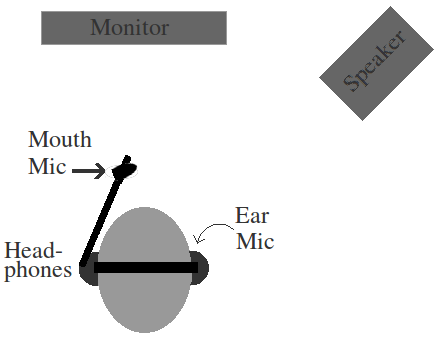
\includegraphics[width=0.45\textwidth]{figure/overallSetUp_new.png}
  \caption{This is the same setup as described in Chapter \ref{chapter2}, except that the mouth microphone is facing the loudspeaker, rather than the mouth.}
  \label{fig:overallSetUp_new}
\end{wrapfigure}
%
It shared the same issue as the omnidirectional microphone, namely that pointing the mouth-microphone toward the loudspeaker, rather than increasing the noise, ignored the fact that the noise level inside the ear canal would likely increase as well with an increase in ambient noise.  Given the alternatives outlined in Section \ref{chap2:limitations}, this was seen as the best available option.  Figures \ref{fig:spectNewMouthNoise} and \ref{fig:spectNewEarNoise} show the new noisy mouth-recorded and ear-recorded speech, respectively.  These are presented along with Figures \ref{fig:spectOldMouthNoise} and \ref{fig:spectOldEarNoise}, the speech collected in the previous experiment in Chapter \ref{chapter2}, for comparison

\begin{figure}[h!]
\begin{subfigure}{0.45\textwidth}
  \centering
  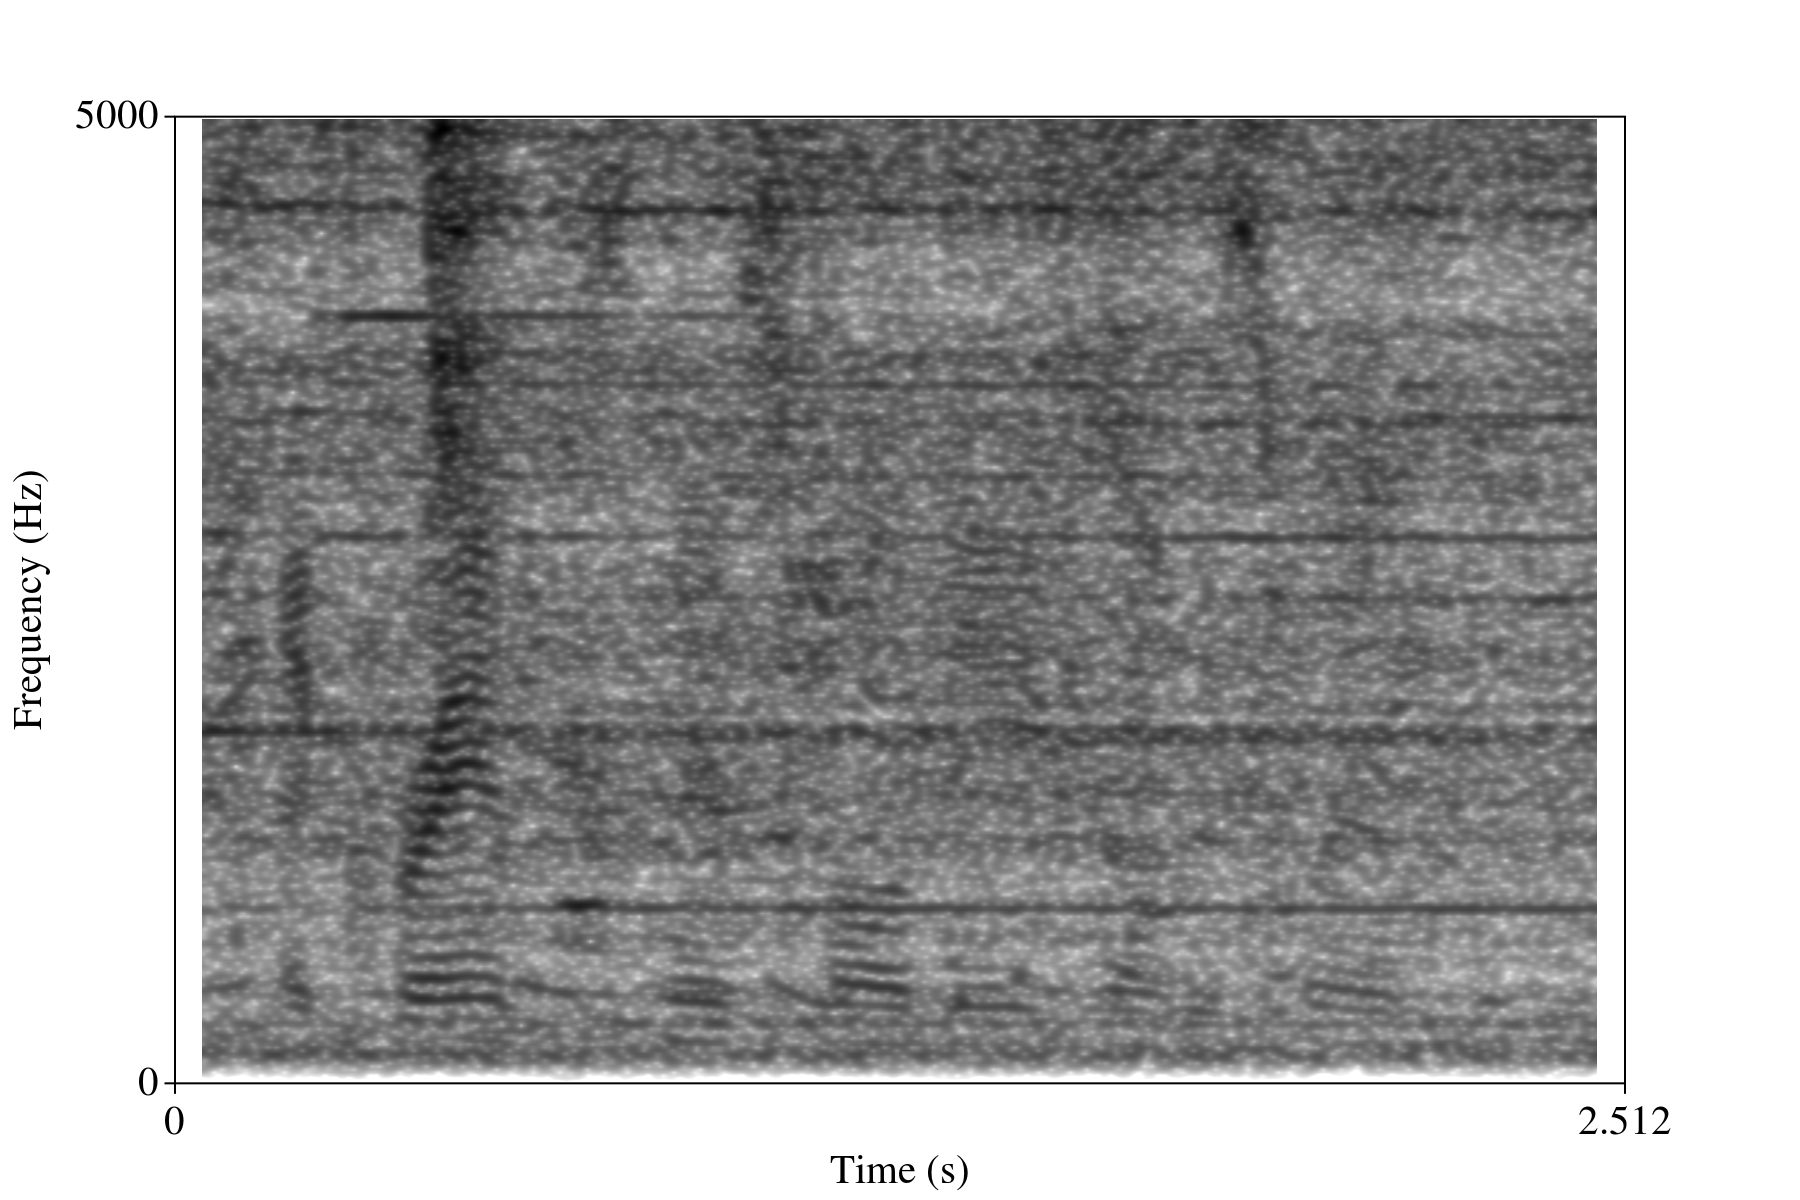
\includegraphics[width=0.9\textwidth]{figure/spectNewMouthNoise.png}
  \caption{New recording at the mouth with the microphone pointed toward the loudspeaker noise source.}
  \label{fig:spectNewMouthNoise}
\end{subfigure}
\qquad
\begin{subfigure}{0.45\textwidth}
  \centering
  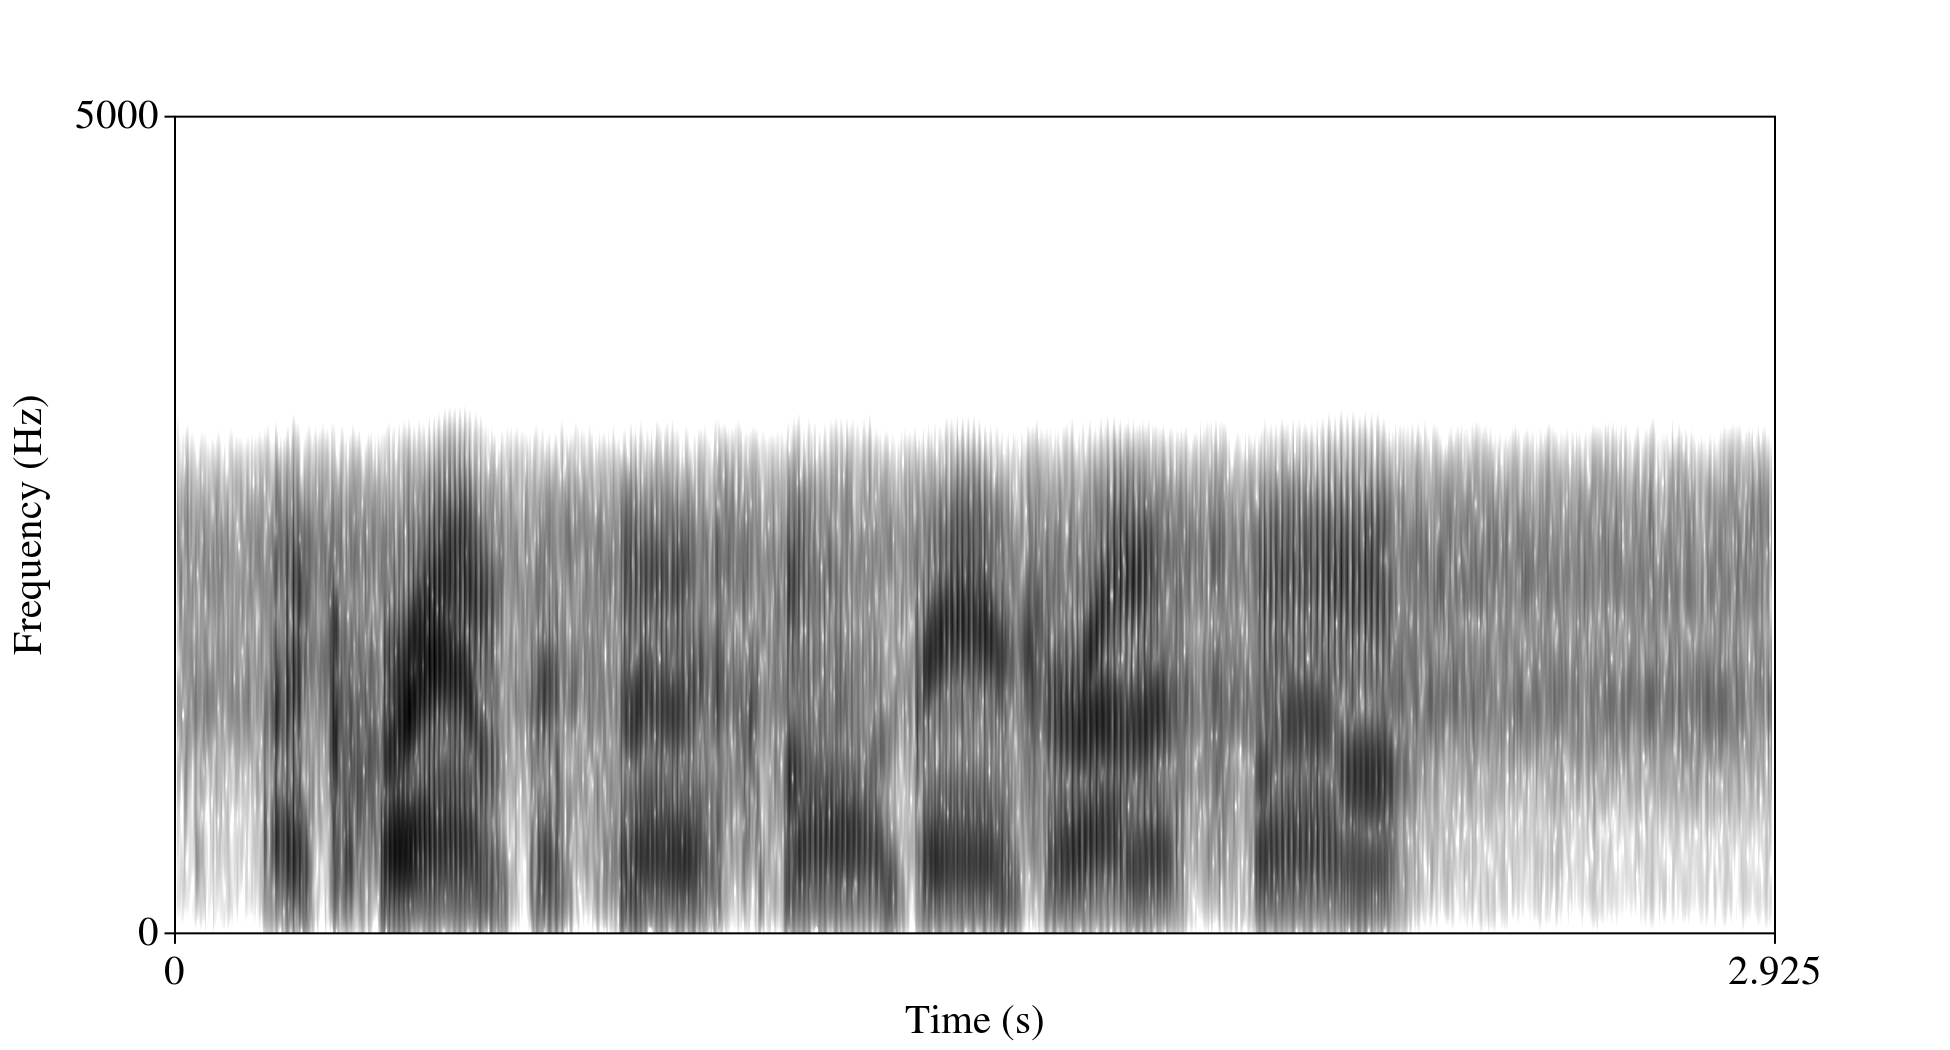
\includegraphics[width=0.9\textwidth]{figure/spectNewEarNoise.png}
  \caption{New recording at the ear; all recording conditions for the ear were the same as in the first group of recordings.}
  \label{fig:spectNewEarNoise}
\end{subfigure}
\\[2ex]
\begin{subfigure}{0.45\textwidth}
  \centering
  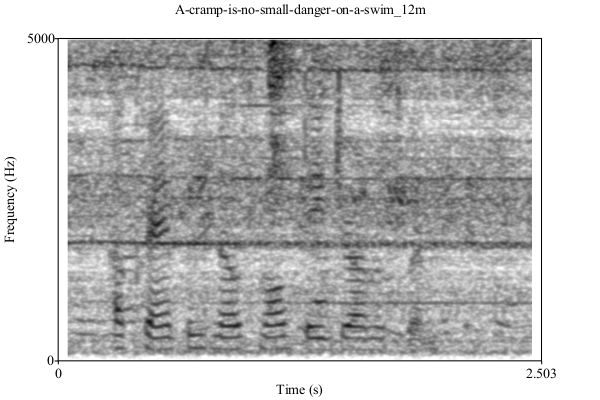
\includegraphics[width=0.9\textwidth]{figure/spctgrmNarrowMthNoise_35.pdf}
  \caption{Recording from the first set of experiments (in Chapter \ref{chapter2}), with the microphone pointed toward the speaker's mouth.}
  \label{fig:spectOldMouthNoise}
\end{subfigure}
\qquad
\begin{subfigure}{0.45\textwidth}
  \centering
  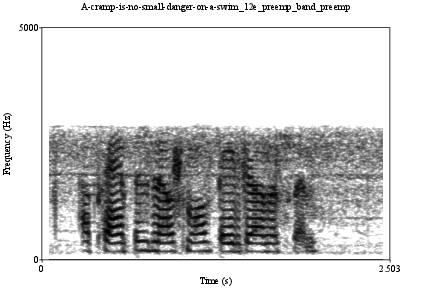
\includegraphics[width=0.9\textwidth]{figure/spctgrmNarrowEarNoisePrempFiltPremp.pdf}
  \caption{Recording at the ear from the first set of experiments (in Chapter \ref{chapter2}); all recording conditions for the ear were the same as in the second group of recordings.}
  \label{fig:spectOldEarNoise}
\end{subfigure}
\caption{The sentence ``A cramp is no small danger on a swim''. In Figs. \ref{fig:spectNewMouthNoise} and \ref{fig:spectNewEarNoise}, spoken by the male speaker, recorded at the mouth with 80 dB `bus' noise and simultaneously at the ear, respectively.  In Figs. \ref{fig:spectOldMouthNoise} and \ref{fig:spectOldEarNoise}, spoken by a female speaker, recorded at the mouth with 80 dB `bus' background noise and simultaneously at the ear, respectively.}
\end{figure}

Note that unlike the previous data collection experiment (cf. Chapter \ref{chapter2}, Section \ref{expt1}), there was only one one noise \textit{level} - 80 dB.  Data for the 60 and 70 dB noise level conditions were not collected for these two speakers.  All previously used background noise types (bus, caf\'{e}, pedestrian area, street, factory) were used for this data collection task as well.

The SNR was calculated for the male speaker using the code specified in Chapter \ref{chapter2} Section \ref{chap2:observations}.  This yielded an average value of slightly below +1 dB SNR for the noisy speech recorded with 80 dB background noise.  This was substantially lower than the 80 dB condition in the data collection experiment with an average SNR of +12 dB.  At that time, the female speaker's SNR was not calculated.  This was later (cf. Sections \ref{chap3:discussion}, \ref{chap3:future-research}) deemed to be an obvious mistake, as the female speaker's SNR was much higher than the male speaker's SNR at approximately +8 dB SNR.  It was likely that the female speaker spoke louder than the male speaker during the experiment, which resulted in the difference.


\subsection{Design}
\label{chap3:methods:design}

The experiment had three factors - gender of speaker\footnote{This was included to test if there is an effect of gender of the speaker on listeners' perception in noise or on transmission of speech through the head and into the ear canal, due to the difference in male and female vocal tract and aural anatomy.} \textbf{x} microphone location \textbf{x} noise type - resulting in a 2x2x6 experiment.  There were two genders (female, male), two mic locations (recording at the ear, recording at the mouth), and six noise types (bus, caf\'{e}, pedestrian, street, factory, and no noise (clean)).  Since the ability to understand speech in noise is quite variable between individuals (cf. \cite{ding:13,gilbert:13}), the design of this experiment was a within-subjects experiment.  This meant that each of the 2x2x6 (ie. 24) conditions needed to be heard by each participant.  The sessions that were re-recorded utilized 80 distinct sentences, which allowed for three sentences to appear in each of the 24 conditions, totaling 72 sentences used in the experiment.  The eight remaining sentences were used as a `training' set intended to get the participants used to the task itself, rather than to acclimate them to the type of speech that they would hear.

Since a given participant could not hear the same sentence twice without introducing a training confound, and since each sentence was recorded in each of the 24 conditions\footnote{72 distinct sentences * 24 conditions = 1728 total sentence recordings}, this necessitated the use of 24 counter-balanced groups to ensure that each one of the 1728 sentences was heard by at least one participant listener.  For example, items (sentences) 1, 2, and 3 occurred in Condition \#1 (eg. female speaker, mic at the mouth, with bus background noise) in counter-balanced group \#1 for Participant \#1. Participant \#2 saw counter-balanced group \#2, which placed items (sentences) 1, 2, and 3 in Condition \#2 (eg. female speaker, mic at the mouth, with caf\'{e} background noise).  Each three-item (sentence) grouping always appeared together in a condition, ie. item (sentence) groupings always appeared together in a counter-balanced group.  

However, once the sentences were assigned to a particular condition, the order of presentation to each participants was randomized; each participant received a different random stimulus order.  Due to the randomized order, it was more difficult for participants to predict the noise type from one sentence to the next, which was intended to slow down the rate at which participants became familiarized with the noise types.

\subsection{Participants}
\label{chap3:methods:participants}

Twenty-four native speakers of English with self-reported normal hearing participated in the experiment. Each participant was placed into a separate counter-balanced group, as specified above in Section \ref{chap3:methods:design}.  This left each counter-balanced group with one participant.

\subsection{Equipment}
\label{chap3:methods:equipment}

The experiment was conducted in a soundbooth with a pair of over-the-ear headphones.  The experiment interface utilized in-house developed software.  The software played the stimulus for the listeners and provided a textbox for them to type their answers.  It placed a time limit on their response, and locked in their answer after 18 seconds if the participant had not already advanced to the next stimulus. The software recorded the participants' answer to each stimulus in a log file.  A computer placed outside the soundbooth, whose monitor could be seen from inside the soundbooth, was used to run the software and displayed the textbox for entering responses.

\subsection{Procedure}
\label{chap3:methods:procedure}

The participant was seated in the sound booth in front of a keyboard and computer monitor\footnote{The computer monitor was outside the soundbooth, and did not produce noise interfering with the task.} with a pair of headphones, and was given a set of instructions. They were told that they would hear each utterance only once, and that each utterance contained only real English words; they were told it was possible for a sentence to not be a `complete' sentence.  The researcher forewarned them that many of the sentences they would hear would be noisy and difficult to understand. They were instructed to write all words they heard, even if what was heard did not make syntactic sense, or if the words were not adjacent (eg. if only the first and last words of the sentence were heard). They were given 18 seconds to type their response, beginning at the onset of the utterance audio, before their answer was locked in.

The participant was told that the first set of eight utterances they heard were part of a `training' set intended to familiarize them with the task. The same eight sentences were heard by every participant.  None of the utterances from the training set were used in the analysis.  Once they they finished the initial set, participants were able to ask if they had any questions.  Afterwards, they began the primary task in the soundbooth.  They would hear one of the sentences, and type their answer in a text box.  When finished with their answer, they would either click to advance to the next sentence, or, if they ran into the time limit, they were prevented from modifying their answer.  The software prompted them to click another button to advance, and did not advance automatically.

After the experiment, the researcher double checked the participant answers for correct spelling.  Only obvious errors were modified (eg. `teh' to `the', `crakers' to `crackers', `mantle' to `mantel'), while ambiguous errors were left as-is (eg. `blo' was not changed to `block', `finde' was not changed to `fine').  Numbers were also lexicalized (eg. `30' to `thirty').  Punctuation was removed for ease of analysis and calculation of word error rate.  Exact responses given by each participant can be found in Appendix F\ref{appendixF}.


\section{Results}
\label{chap3:results}

\begin{kframe}


{\ttfamily\noindent\itshape\color{messagecolor}{\#\# The following objects are masked from mydata (pos = 3):\\\#\# \\\#\#\ \ \ \  group, mic\_location, noise\_type, sentence, sentence\_number,\\\#\#\ \ \ \  speaker\_gender, subject, wer\\\#\# \\\#\# The following objects are masked from mydata (pos = 3):\\\#\# \\\#\#\ \ \ \  group, mic\_location, noise\_type, sentence, sentence\_number,\\\#\#\ \ \ \  speaker\_gender, subject, wer}}

{\ttfamily\noindent\itshape\color{messagecolor}{\#\# The following objects are masked from mydata (pos = 4):\\\#\# \\\#\#\ \ \ \  group, mic\_location, noise\_type, sentence, sentence\_number,\\\#\#\ \ \ \  speaker\_gender, subject, wer}}

{\ttfamily\noindent\itshape\color{messagecolor}{\#\# The following objects are masked from mydata (pos = 3):\\\#\# \\\#\#\ \ \ \  group, mic\_location, noise\_type, sentence, sentence\_number,\\\#\#\ \ \ \  speaker\_gender, subject, wer}}

{\ttfamily\noindent\itshape\color{messagecolor}{\#\# The following objects are masked from mydata (pos = 4):\\\#\# \\\#\#\ \ \ \  group, mic\_location, noise\_type, sentence, sentence\_number,\\\#\#\ \ \ \  speaker\_gender, subject, wer}}

{\ttfamily\noindent\itshape\color{messagecolor}{\#\# The following objects are masked from mydata (pos = 5):\\\#\# \\\#\#\ \ \ \  group, mic\_location, noise\_type, sentence, sentence\_number,\\\#\#\ \ \ \  speaker\_gender, subject, wer}}

{\ttfamily\noindent\itshape\color{messagecolor}{\#\# The following objects are masked from mydata (pos = 3):\\\#\# \\\#\#\ \ \ \  group, mic\_location, noise\_type, sentence, sentence\_number,\\\#\#\ \ \ \  speaker\_gender, subject, wer}}

{\ttfamily\noindent\itshape\color{messagecolor}{\#\# The following objects are masked from mydata (pos = 4):\\\#\# \\\#\#\ \ \ \  group, mic\_location, noise\_type, sentence, sentence\_number,\\\#\#\ \ \ \  speaker\_gender, subject, wer}}

{\ttfamily\noindent\itshape\color{messagecolor}{\#\# The following objects are masked from mydata (pos = 5):\\\#\# \\\#\#\ \ \ \  group, mic\_location, noise\_type, sentence, sentence\_number,\\\#\#\ \ \ \  speaker\_gender, subject, wer}}

{\ttfamily\noindent\itshape\color{messagecolor}{\#\# The following objects are masked from mydata (pos = 6):\\\#\# \\\#\#\ \ \ \  group, mic\_location, noise\_type, sentence, sentence\_number,\\\#\#\ \ \ \  speaker\_gender, subject, wer}}

{\ttfamily\noindent\color{warningcolor}{\#\# Warning: Collapsing data to cell means. *IF* the requested effects are a subset of the full design, you must use the "{}within\_full"{} argument, else results may be inaccurate.}}

{\ttfamily\noindent\color{warningcolor}{\#\# Warning: You have removed one or more levels from variable "{}noise\_type"{}. Refactoring for ANOVA.}}

{\ttfamily\noindent\color{warningcolor}{\#\# Warning: Collapsing data to cell means. *IF* the requested effects are a subset of the full design, you must use the "{}within\_full"{} argument, else results may be inaccurate.}}

{\ttfamily\noindent\color{warningcolor}{\#\# Warning: You have removed one or more levels from variable "{}noise\_type"{}. Refactoring for ANOVA.}}\end{kframe}

The word error rate (WER) for each (spell-checked) response for each participant was calculated. The code for the WER calculation can be found in Appendix F\ref{appendix?}

A 3-way, within-subjects ANOVA was performed with the collected data - 72 sentences from each of the 24 participants. Factors included the gender (of the speaker of the pre-recorded stimulus; male, female), the recording (mic) location (at the mouth, at the ear), and background noise type (no noise, bus, caf\'{e}, pedestrian area, street, factory) - 2\textbf{x}2\textbf{x}6 design.  WER was the dependent variable.  An ANOVA was chosen to test for statistical significance over an LME due to the large number of conditions in the study; the reported results from the ANOVA were much more concise, whereas the LME would have required a substantial amount of re-leveling comparison tests.  

By-subjects ($S$) and by-items ($I$) ANOVAs were performed (cf. Table \ref{tab:anova1}). Mauchley's Test for Sphericity\footnote{Sphericity assumes that the variance of the differences between all pairs of conditions is the same; sphericity is violated when this is not the case.} was conducted, both for the by-subjects and by-items ANOVAs.  Significant sphericity violations were found for the main effect of noise type, and the interaction of speaker gender and noise type.  These were corrected for using a Greenhouse-Geisser test, but they resulted in no change to statistical significance.  The values below incorporate the corrections.

% ($F_1$($by_subj_ez_anova$ANOVA$DFn[6]$,$by_subj_ez_anova$ANOVA$DFd[6]$) = $by_subj_ez_anova$ANOVA$F[6]$, $p>0.1$; $F_1$($by_items_ez_anova$ANOVA$DFn[6]$,$by_items_ez_anova$ANOVA$DFd[6]$) = $by_items_ez_anova$ANOVA$F[6]$, $p>0.05$)

The main effects of all three factors were significant (cf. Table \ref{tab:anova1}).  Two, two-way interactions were significant: speaker gender \textbf{x} mic location, and noise-type \textbf{x} mic location. The two way interaction between speaker gender and noise type was not significant, nor was the three-way interaction between speaker gender, mic location, and noise type.
  

% latex table generated in R 3.4.1 by xtable 1.8-2 package
% Tue Aug  1 22:29:00 2017
\begin{table}[ht]
\centering
\begin{tabular}{llrrrrl}
  \hline
ANOVA & Effect & DFn & DFd & F & p & * \\ 
  \hline
S & speaker\_gender & 1 & 23 & 6.69 & 0.02 & * \\ 
  I & speaker\_gender & 1 & 71 & 4.01 & 0.05 & * \\ 
  S & noise\_type & 5 & 115 & 84.83 & 0.00 & * \\ 
  I & noise\_type & 5 & 355 & 103.50 & 0.00 & * \\ 
  S & mic\_location & 1 & 23 & 155.07 & 0.00 & * \\ 
  I & mic\_location & 1 & 71 & 354.53 & 0.00 & * \\ 
  S & speaker\_gender:noise\_type & 5 & 115 & 0.55 & 0.74 &  \\ 
  I & speaker\_gender:noise\_type & 5 & 355 & 0.52 & 0.76 &  \\ 
  S & speaker\_gender:mic\_location & 1 & 23 & 18.53 & 0.00 & * \\ 
  I & speaker\_gender:mic\_location & 1 & 71 & 21.36 & 0.00 & * \\ 
  S & noise\_type:mic\_location & 5 & 115 & 55.53 & 0.00 & * \\ 
  I & noise\_type:mic\_location & 5 & 355 & 71.03 & 0.00 & * \\ 
  S & speaker\_gender:noise\_type:mic\_location & 5 & 115 & 1.61 & 0.16 &  \\ 
  I & speaker\_gender:noise\_type:mic\_location & 5 & 355 & 1.86 & 0.10 &  \\ 
   \hline
\end{tabular}
\caption{ANOVA for by-subjects (S) and by-items (I) analysis of the three-factor, within-subjects experiment. `ANOVA' indicates by-subject (S) or by-item (I) analysis, `Effect' lists the factor(s) tested, `DFn' and `DFd' refer to the degrees of freedom numerator and denominator, `F' is the F-score, `p' is the p-value, and `*' marks a significant p-value.} 
\label{tab:anova1}
\end{table}



% Mauchley's Test for Sphericity\footnote{Sphericity assumes that the variance of the differences between all pairs of conditions is the same; sphericity is violated when this is not the case.} was conducted, both for the by-subjects and by-items ANOVAs.  Significant sphericity violations were found for the main effect of noise type, and the interaction of speaker gender and noise type, as can be seen in Tables \ref{tab:anova1_subj_sph_test} and \ref{tab:anova1_item_sph_test}. 
% 
% <<ANOVA1_sphericity_test, echo=FALSE, results='asis'>>=
% print(xtable(by_subj_ez_anova$`Mauchly's Test for Sphericity`, label="tab:anova1_subj_sph_test", caption="Sphericity test for the by-subjects ANOVA."), include.rownames=FALSE)
% print(xtable(by_item_ez_anova$`Mauchly's Test for Sphericity`, label="tab:anova1_item_sph_test", caption="Sphericity test for the by-items ANOVA."), include.rownames=FALSE)
% by_subj_ez_anova$`Sphericity Corrections`$HFe <- NULL
% by_item_ez_anova$`Sphericity Corrections`$HFe <- NULL
% by_subj_ez_anova$`Sphericity Corrections`$`p[HF]` <- NULL
% by_item_ez_anova$`Sphericity Corrections`$`p[HF]` <- NULL
% by_subj_ez_anova$`Sphericity Corrections`$`p[HF]<.05` <- NULL
% by_item_ez_anova$`Sphericity Corrections`$`p[HF]<.05` <- NULL
% @
% 
% The corrections for sphericity were performed using a Greenhouse-Geisser test, for both by-subjects (Table \ref{tab:anova1_subj_sph_corr}) and by-items (Table \ref{tab:anova1_item_sph_corr}) ANOVAs.  Neither resulted in a change to any prior finding.
% 
% <<ANOVA1_sphericity_corr, echo=FALSE, results='asis'>>=
% print(xtable(by_subj_ez_anova$`Sphericity Corrections`, label="tab:anova1_subj_sph_corr", caption="Sphericity corrections for the by-subjects ANOVA."), include.rownames=FALSE)
% print(xtable(by_item_ez_anova$`Sphericity Corrections`, label="tab:anova1_item_sph_corr", caption="Sphericity corrections for the by-subjects ANOVA."), include.rownames=FALSE)
% @
% Noting the sphericity violations involving the noise type condition, the data was viewed in the box plots in Figures \ref{fig:anova1_noise_boxplot}, \ref{fig:anova1_noiseXspkr_boxplot}, and \ref{fig:anova1_noiseXmic_boxplot}.
% When viewing the simple effects of noise in Figure \ref{fig:anova1_noise_boxplot}, it is apparent (and intuitive) that the no-noise condition differs distinctly from the other noise types.
% 
% This holds true when viewing the interaction of speaker gender \textbf{x} noise type in 
% %
% \begin{wrapfigure}{l!}{0.5\textwidth}
% <<boxplot_noise, echo=FALSE, results='asis'>>=
% par(mar=c(7,5,0,0))
% boxplot(wer~noise_type,col=c("white","lightgray"),mydata, las=2, names=c("No Noise","Bus","Cafe","Pedestrian","Street","Factory"),ylab="WER", cex.axis=1.5, cex.lab=2.0)
% @
% \caption{Boxplot displaying the average word error rate (WER) averaged over each participant for every noise type. WER is the variable on the y-axis, and noise type is on the x-axis.}
% \label{fig:anova1_noise_boxplot}
% \end{wrapfigure}
% %
% Figure \ref{fig:anova1_noiseXspkr_boxplot} and the interaction of noise type \textbf{x} mic location in Figure \ref{fig:anova1_noiseXmic_boxplot}.  The conditions in which there is no noise present differ noticeably from those with noise; this can visually be seen even in the condition in which the speech was recorded at the ear. This is likely the root of the sphericity violations.
% 
% %\begin{wrapfigure}{L}{1\textwidth}
% \begin{figure}[h!]
% <<boxplot_noiseXspkr, echo=FALSE, results='asis'>>=
% boxplot(wer~noise_type*speaker_gender,col=c("white","lightgray"),mydata, names=c("Female\nNo Noise","Female\nBus","Female\nCafe","Female\nPedestrian","Female\nStreet","Female\nFactory","Male\nNo Noise","Male\nBus","Male\nCafe","Male\nPedestrian","Male\nStreet","Male\nFactory"),ylab="WER",las=2)
% @
% \caption{Boxplot displaying the average word error rate (WER) averaged over each participant for the interaction of every noise type by the speaker gender. WER is the variable on the y-axis, and noise type by speaker gender is on the x-axis.}
% \label{fig:anova1_noiseXspkr_boxplot}
% \end{figure}
% 
% \begin{figure}[h!]%{L}{\textwidth}
% <<boxplot_noiseXmic, echo=FALSE, results='asis'>>=
% boxplot(wer~noise_type*mic_location,col=c("white","lightgray"),mydata, names=c("Ear\nNo Noise","Ear\nBus","Ear\nCafe","Ear\nPedestrian","Ear\nStreet","Ear\nFactory","Mouth\nNo Noise","Mouth\nBus","Mouth\nCafe","Mouth\nPedestrian","Mouth\nStreet","Mouth\nFactory"),ylab="WER",las=2)
% @
% \caption{Boxplot displaying the average word error rate (WER) averaged over each participant for the interaction of every noise type by the mic location. WER is the variable on the y-axis, and noise type by mic location is on the x-axis.}
% \label{fig:anova1_noiseXmic_boxplot}
% \end{figure}


The factor of speaker gender was split, and two two-way ANOVA were calculated for each level of speaker gender (female, male) with factors of noise type and microphone location.  Both by-subjects and by-items ANOVA, for both female and male speakers, found the noise type \textbf{x} microphone location interaction significant and both main effects of noise type and microphone location significant, with $p<0.005$ in all conditions.  The simple effects of microphone location were calculated, for each combination of speaker gender and noise type, and all were found to be significant, with $p<0.005$ in all conditions.  The simple effects of noise type were calculated.  For all female gender conditions (mic at the ear and at the mouth), and for the male gender condition with the microphone at the mouth, all effects are significant with $p<0.005$.  However, for the male gender condition with the microphone at the ear, there was no significant effect of noise, including the `no noise' condition ($F_{subj}(5,115)=2.01, p>0.05$; $F_{item}(5,355)=2.25, p<0.05$).

Since there is a statistical difference in the main effect of noise, and since the `no noise' condition is expected to contain different WERs from the other noise conditions, another ANOVA was calculated with the `no noise' level of noise type removed.  This was to test for statistical difference only in noise conditions containing actual noise (and any resulting interaction). This modified ANOVA is a 2 \textbf{x} 2 \textbf{x} 5 design, with the noise type factor only having 5 levels (with the `no noise' condition removed from the noise type factor).  As before, the values below include Greenhouse-Geisser corrections for Sphericity violations for noise type, but this resulted in no change to any significant values.

There are significant main effects of noise type and mic location (cf. Table \ref{tab:anova2}).  The main effect of speaker gender is only significant in the by-subjects ANOVA, but is not significant in the by-items ANOVAs.  There are two significant two-way interactions of speaker gender \textbf{x} mic location and noise type \textbf{x} mic location, but no significant interaction of speaker gender \textbf{x} noise type, and no significant three-way interaction.  

% latex table generated in R 3.4.1 by xtable 1.8-2 package
% Tue Aug  1 22:29:01 2017
\begin{table}[ht]
\centering
\begin{tabular}{llrrrrl}
  \hline
ANOVA & Effect & DFn & DFd & F & p & * \\ 
  \hline
S & speaker\_gender & 1 & 23 & 5.26 & 0.03 & * \\ 
  I & speaker\_gender & 1 & 71 & 3.46 & 0.07 &  \\ 
  S & noise\_type & 4 & 92 & 5.95 & 0.00 & * \\ 
  I & noise\_type & 4 & 284 & 6.92 & 0.00 & * \\ 
  S & mic\_location & 1 & 23 & 215.08 & 0.00 & * \\ 
  I & mic\_location & 1 & 71 & 515.73 & 0.00 & * \\ 
  S & speaker\_gender:noise\_type & 4 & 92 & 0.60 & 0.66 &  \\ 
  I & speaker\_gender:noise\_type & 4 & 284 & 0.55 & 0.70 &  \\ 
  S & speaker\_gender:mic\_location & 1 & 23 & 16.68 & 0.00 & * \\ 
  I & speaker\_gender:mic\_location & 1 & 71 & 20.62 & 0.00 & * \\ 
  S & noise\_type:mic\_location & 4 & 92 & 6.00 & 0.00 & * \\ 
  I & noise\_type:mic\_location & 5 & 355 & 71.03 & 0.00 & * \\ 
  S & speaker\_gender:noise\_type:mic\_location & 4 & 92 & 1.14 & 0.34 &  \\ 
  I & speaker\_gender:noise\_type:mic\_location & 4 & 284 & 1.35 & 0.25 &  \\ 
   \hline
\end{tabular}
\caption{ANOVA for by-subjects (S) and by-items (I) analysis of the three-factor, within-subjects experiment; the level of `no noise' has been removed from the noise type factor. `ANOVA' indicates by-subject (S) or by-item (I) analysis, `Effect' lists the factor(s) tested, `DFn' and `DFd' refer to the degrees of freedom numerator and denominator, `F' is the F-score, `p' is the p-value, and `*' marks a significant p-value.} 
\label{tab:anova2}
\end{table}


As before, the factor of gender was split, and two two-way ANOVAs were run for the factors of noise type and microphone location, at each level of speaker gender (female, male).  The ANOVA with the male data has significant main effects of noise and microphone location, with $p<0.005$ in all conditions, but there was no significant interaction of noise type and microphone location ($F_{subj}(4,92)=1.54, p>0.1$; $F_{item}(4,284)=2.11, p>0.05$).  The ANOVA for the female data contained a significant main effect of microphone location ($F_{subj}(1,23)=107.31, p<0.001$; $F_{item}(1,71)=130.26, p<0.001$) and a significant interaction of microphone location \textbf{x} noise type ($F_{subj}(4,92)=5.2, p<0.005$; $F_{item}(4,284)=3.51, p<0.001$), but no main effect of noise type ($F_{subj}(4,92)=2.63, p>0.05$; $F_{item}(4,284)=2.66, p<0.05$).

The simple effects for microphone location were calculated, and as before, all were significant with $p<0.005$.  The simple effects of noise were calculated, and there were significant effects of noise type for both levels of gender with the microphone at the mouth, $p<0.005$.  However, there were no significant effects of noise (again, this test excludes the `no noise' condition) for either gender when the microphone was placed in the ear (female: ($F_{subj}<1; F_{item}<1$); male: ($F_{subj}(4,92)=1.06, p>0.1$; $F_{item}(4,284)=1.10, p>0.1$)).


% 
% Again, Mauchley's Test for Sphericity was conducted, resulting only in a significant sphericity violation in the by-subjects ANOVA for noise (cf. Tables \ref{tab:anova2_subj_sph_test} and \ref{tab:anova2_item_sph_test}).  This was corrected with a Greenhouse-Geisser test, which resulted, again, in no changes to the determinations of statistical significance indicated in the ANOVAs in Tables \ref{tab:anova2_by_subj} and \ref{tab:anova2_by_item}.
% <<ANOVA2_sphericity_test, echo=FALSE, results='asis'>>=
% print(xtable(by_subj_ez_anova2$`Mauchly's Test for Sphericity`, label="tab:anova2_subj_sph_test", caption="Sphericity test for the by-subjects ANOVA with the `no noise' condition removed."), include.rownames=FALSE)
% print(xtable(by_item_ez_anova2$`Mauchly's Test for Sphericity`, label="tab:anova2_item_sph_test", caption="Sphericity test for the by-items ANOVA with the `no noise' condition removed."), include.rownames=FALSE)
% by_subj_ez_anova2$`Sphericity Corrections`$HFe <- NULL
% by_item_ez_anova2$`Sphericity Corrections`$HFe <- NULL
% by_subj_ez_anova2$`Sphericity Corrections`$`p[HF]` <- NULL
% by_item_ez_anova2$`Sphericity Corrections`$`p[HF]` <- NULL
% by_subj_ez_anova2$`Sphericity Corrections`$`p[HF]<.05` <- NULL
% by_item_ez_anova2$`Sphericity Corrections`$`p[HF]<.05` <- NULL
% @
% 
% 
% %(cf. Tables \ref{tab:anova2_subj_sph_corr} and \ref{tab:anova2_item_sph_corr}).
% 
% % # <<ANOVA2_sphericity_corr, echo=FALSE, results='asis'>>=
% % # print(xtable(by_subj_ez_anova2$`Sphericity Corrections`, label="tab:anova2_subj_sph_corr", caption="Sphericity corrections for the by-subjects ANOVA with the ``no noise'' condition removed."), include.rownames=FALSE)
% % # print(xtable(by_item_ez_anova2$`Sphericity Corrections`, label="tab:anova2_item_sph_corr", caption="Sphericity corrections for the by-items ANOVA with the ``no noise'' condition removed."), include.rownames=FALSE)
% % # @




\section{Discussion}\label{chap3:discussion}

% Points to hit here:
% X- Ear speech is more easily recognized than noisy speech from the mouth (print bar graph of mic loc simple effects)
% X- There is still a main effect of noise even when 'no noise' is removed, print bar graph w/ no 'no noise' and discuss simple effects
% X- Touch on 'near-significance' of speaker gender, how it isn't as near significant as it appears - likely an SNR effect (print graph).
% - Discuss noiseXmic interation data, re-print graph
% X-- Mention differences in mouth noise performance which come out in this interaction, medians ranging from approximately 60% (factory) to near 90% (bus); reference noise spectograms, give possible explanation
% X-- Non-noisy mouth speech is still the most easily recognized - median of zero - but non-noisy ear-speech does well for itself with a median nearing 15% WER.
% X-- There still appears to be a noticeable difference between ear-no noise and ear-noisy speech (some noise must get through), but no noticeable difference between noises within ear-speech category; nevertheless, median noisy ear-speech recognition appears to hover near 30% WER.
% X-- Comment on how this is evidence for ''predictable'' noise that is (more or less) non-varying between noise types.
% X- Look at longitudinal effects
% -- Surveys - add in later
% X- Move on to limitations
% -- Mention not all sound files had normalized amplitude - some were quite louder than others, which may be an explanation for some of the observed variability.
% -- Mention the computer screen distraction.


The primary hypotheses from Chapter \ref{chapter2} included (a) that the signal recorded from the ear, pre-emphasized, filtered, and pre-emphasized again, would be intelligible by human listeners, and (b) that it would be more intelligible than speech with a noisy background, ie. that environmental noise would have very little effect on the signal.  The results in Section \ref{chap3:results} above show a statistical difference between the WERs of the sentence transcriptions of the speech recorded in every simple effect of microphone location in every condition, ie. recognition of speech recorded form the ear canal is statistically different than the recognition of speech recorded at the mouth in the tested conditions.  This can be seen more clearly in the graphs containing all levels of data, Figures \ref{fig:female-split} and \ref{fig:male-split}.  The noisy (non-clean) speech recorded at the ear has a significantly lower transcription WER than the noisy speech recorded at the mouth, splitting over all noise conditions.  This finding seems to validate hypothesis (b), that noise has does not have as much of an effect on the ear-recorded signal as it does on the mouth recorded signal.

There is a significant simple effect of microphone location at the level of `no noise', as well.  The effect goes in the opposite direction, as the clean ear-recorded speech has a \textit{higher} WER than the clean mouth-recorded speech.  This appears to give a partial validation of hypothesis (a); while the ear-recorded speech is intelligible by human listeners, is is not \textit{as} intelligible as mouth-recorded speech with little or no noise.

Out of all condition combinations in Figures \ref{fig:female-split} and \ref{fig:male-split}, the WER front-runner is quite clearly the speech recorded at the mouth with no background noise.  There was never any doubt that this would be the case, as speech with a \textit{relatively} high SNR is the sort of speech whereby most communication occurs (ie. not with consistent 80 dB background noise, nor with significantly low-pass filtered speech).  The median WER is, unsurprisingly, 0\%, though there is some variance from perfect perception; some errors do occasionally occur. The ear-recorded speech in a clean environment manages to also achieve a respectable transcription WER median of approximately 15\% for both the male- and female-spoken stimuli, with a lower quartile boundary at 0\% WER and an upper quartile boundary of approximately 35\% WER.


\begin{figure}[h!]

\includegraphics[width=\maxwidth]{figure/All-Factors-Female-1} 

\caption{Comparison of ear-recorded and mouth-recorded speech at every level of noise type, for the female-spoken stimuli.  White bars signify ear-recorded speech, and grey bars signify mouth-recorded speech.}\label{fig:female-split}
\end{figure}

\begin{figure}[h!]

\includegraphics[width=\maxwidth]{figure/All-Factors-Male-1} 

\caption{Comparison of ear-recorded and mouth-recorded speech at every level of noise type, for the male-spoken stimuli.  White bars signify ear-recorded speech, and grey bars signify mouth-recorded speech.}\label{fig:male-split}
\end{figure}

% 0Discuss Mic vs Ear results basic

Despite being more similar than their mouth recorded counterparts, there is still an observable difference between the ear recorded speech with no noise, and ear recorded speech in noisy conditions.  Most noise conditions recorded from the ear achieve a lower quartile boundary near 0\%, but the upper quartile boundary for most nears 60\% WER.  The median WER for noise conditions generally falls at or slightly below 30\%. 
Even though there is a higher WER than the ear-recorded no-noise condition, the ear-recorded speech in noise appears to be quite consistent across noise categories.  This is very different from the mouth-recorded speech in noise, which vary considerably between noise conditions. Again, this trends toward supporting hypothesis (b), that noise presence and noise type will have a statistically greater effect on mouth-recorded speech than ear-recorded speech.

% 1Discuss significant interaction of noise and mic, and significant simple effect of noise for all mic locs except ear for male
These observations are backed by the statistical results.  There was also a statistical interaction of noise type \textbf{x} microphone location, and this remained even when the `clean' condition was removed from the dataset, except the interaction disappears when only the male-spoken data is tested after being split by gender.  In looking at the simple effect of noise for the mouth-recorded level of microphone location, there is a statistical difference for both genders, both when the `clean' condition is left in the analysis as well as when it is removed.  This is both clear in Figures \ref{fig:female-split} and \ref{fig:male-split} and intuitive; different types of noise with different qualities will affect recognition in different ways.  This can be contrasted with the simple effects of noise for both genders at the ear (excluding the `clean' condition); there is no statistical difference in recognition (WER) across the levels of noise when the the speech was recorded from the ear.  This indicates that while a noise presence hampers transcription ability and increases WER in ear-recorded conditions, the varying qualities of the different background noises were dampened to the point of having a significantly lesser effect than that which occurs in the mouth-recorded speech.

For the male-spoken data, this trend continued when the `clean' condition was included in the analysis.  There was no simple effect of noise, ie. no statistical difference between any of the noise levels, including `clean' speech, when the speech was recorded at the ear.  This differs from the recognition of the female-spoken speech, which finds a statistical difference of noise type when the `clean' condition is included versus when it is not.  This indicates that some level of noise must be present in the ear-recorded signal in order for a statistical difference to be elicited.  It is worth noting that the female speaker's hair introduced a potential compromise to the seal of the earmuffs used in the experiment (cf. Appendix A\ref{appendixA}), which may be able to explain the gender difference. Emphasizing what is written above, there is still no difference of noise type when the `clean' condition is removed from the analysis.

Regarding the simple effects of noise at the mouth, as previously mentioned, there are statistical effects found for both genders, regardless of whether `clean' speech is included in the analysis.  This demonstrates that the different noise types have different effects on human speech recognition.  The exact reasons why performance differs for different levels of noise is not a primary concern of this study.  The different levels were primarily included to test the above effect, ie. \textit{whether} performance differs with noise type when speech is recorded at the mouth (it does), and \textit{whether} it differs for different noise types when recorded at the ear (it does not).   Visually, in Figures \ref{fig:female-split} and \ref{fig:male-split}, the bus noise condition appears to be the most difficult background noise from which to parse speech, and the factory background noise appears to be the easiest.  Further analysis of these particular differences is not pursued.



% 4Talking about Speaker Gender X Mic Loc interaction, and different dB SNR.  Highlight the differences in the plots above, especially the clean condition
A statistical interaction of speaker gender \textbf{x} mic location is found in both ANOVAs, with the `clean' noise condition and without.  
Looking at the boxplots in Figures \ref{fig:female-split} and \ref{fig:male-split}, it can be visualized that gender affects the recognition of speech at each of the recording locations differently (in the ear, in front of the mouth).  Based on this plot, it would appear that the female ear-recorded speech offers less intelligibility \textit{benefit} over the speech recorded at the mouth, while the male voice offers more benefit. It was previously mentioned that one possibility for the drop in performance of the female, ear-recorded speech was that there was a potential earmuff seal compromise due to the participant's hair.  

It is also very possible that ear-recorded speech by females does not result in as high of recognition performance as that of male-speech.  One simple hypothesis is that there are fewer harmonics in female-speech than in male-speech below the low-pass filter cutoff.  It may also be due to differences in the anatomy of the head, although it is unlikely due to ear canal size, as the size of the outer ear canal recorded for both speakers was rather similar (male speaker: 1.4 mL; female speaker: 1.6 mL)\footnote{Cf. Appendix A\ref{appendixA}}.  These have potential implications for hypothesis (a), that speech recorded at the ear is intelligible, and this difference should be investigated further.
%
% \begin{wrapfigure}{R}{0.5\textwidth}
% <<Mic-location_simple, echo=FALSE, results='asis'>>=
% par(mar=c(4,5,0,0))
% boxplot(wer~mic_location,col=c("white","lightgray"),mydata, names=c("Ear-Recorded","Mouth-Recorded"),ylab="WER", cex.axis=1.5, cex.lab=2.0)
% @
% \caption{Simple effects of Microphone Location.}
% \label{fig:mic_loc_simple}
% \end{wrapfigure}
%

There is also a difference between both genders for speech recorded at the mouth.
However, recall that - in the instance of these two particular speakers - gender is confounded with SNR.  The average female speaker's SNR for noisy, mouth-recorded speech was higher than the male speaker's SNR for noisy, mouth-recorded speech.  As previously mentioned in Section \ref{chap3:methods:design}, the only noise level used for the stimuli in this task was 80 dB; this was constant for both participants, and so it was likely that the female participant spoke louder than the male participant.  The male speaker averaged less than +1 dB SNR and the female speaker averaged over +8 dB SNR, using the SNR calculation script mentioned previously in Section \ref{chap2:observations} and found in Appendix E\ref{appendixE}.

This difference in SNR likely partially contributed to the observed statistical interaction.  If the SNR is high (as it was for the noisy, mouth-recorded female speech), the human auditory system can utilize the methods it has to `release the masking' in an effective manner.  The likelihood that the observed statistical difference was caused by the two speakers' differing SNRs makes sense, as the major difference in listener performance between the two speaker genders occurs within the noisy, mouth-recorded speech (cf. Figs. \ref{fig:female-split} and \ref{fig:male-split}).  Unfortunately, as gender is confounded with SNR, this can only be speculated.



% A closer look at the main effect of noise-type, excluding the level of `no noise', can be seen in Figure \ref{fig:noise-type_non-no-noise_main}.
% 
% The difference here is not nearly as stark as that seen within the microphone location distinction in Figure \ref{fig:mic_loc_simple}.  Still, there is a observable difference, particularly between the bus background noise (with the highest relative WER) and the factory background noise (with the lowest relative WER).
% 
% Referring back to Figure \ref{fig:bkgrnd-noises}, containing the spectograms of the background noises in Section \ref{bkgrnd:speech_in_noise}, it appears that the bus noise (cf. Figure \ref{fig:fac-bkgrnd}) contains bands in the frequency spectrum that contain higher amplitude.
% This may adversely affect a person's ability to parse the harmonics and/or formants from the desired speech. 
% 
% Again referring to Figure \ref{fig:bkgrnd-noises}, it is unclear, however, why the caf\'{e} background noise, among the other noises, has a relatively lower WER, since it also contains many more prominent bands of frequency from speaker babble. 
% Similarly, it is difficult to observe much difference between the factory background noise and the pedestrian background noise, despite the pedestrian noise having a higher upper bound.
% 
% To see if any more apparent differences can be found, Figure \ref{fig:noiseXmic2} shows the noise type factor split between the two levels of mic location, displaying what was originally seen above in Figure \ref{fig:anova1_noiseXmic_boxplot}.  
%
% \begin{wrapfigure}{l}{0.5\textwidth}
% <<spkr-gender_mic-location_interaction, echo=FALSE, results='asis'>>=
% par(mar=c(8,5,0,0))
% boxplot(wer~mic_location*speaker_gender,col=c("white","lightgray"),mydata2, names=c("Female\nEar-Rec.","Female\nMouth-Rec.","Male\nEar-Rec.","Male\nMouth-Rec."),ylab="WER", cex.axis=1.5, cex.lab=2.0, las=2)
% @
% \caption{Interaction between speaker gender and microphone location.}
% \label{fig:spkr-genXmic-loc}
% \end{wrapfigure}
%
% When only looking at the noise as it occurs in the mouth-recorded condition, the differences between the levels of noise become much more stark.  In particular, the difference between the bus noise (high WER) and factory noise (relatively lower WER) greatly expands. 

% This distinction reaches as low as a median of approximately 60\% WER for the factory background noise conditions, and a median of nearly 90\% WER for the bus background noise.  The variance within noise conditions also differs, with the bus noise containing less variance (upper quartile 100\% WER, lower quartile ~68\% WER) than the factory noise condition (upper quartile ~90\% WER, lower quartile ~30\% WER).  The remaining noise conditions are more similar to one another, and fall in between the two, with median WERs hovering near 80\%.  The bus noise, as seen in Figure \ref{fig:bkgrnd-noises}, seems to contain very prominent frequency bands within the frequency range that is important for speech; it is possible that this plays a role in its noticeably higher WER.
% 
% The differences between the transcription WERs of the caf\'{e}, pedestrian, and street noises have expanded slightly, but still hover fairly close together in between the bus and factory performances. No explanation is proposed for the reason for these apparent divergences.


% %
% \begin{wrapfigure}{l}{0.5\textwidth}
% <<Noise-type_simple, echo=FALSE, results='asis'>>=
% par(mar=c(7,5,0,0))
% noiseless_data <- subset(mydata, noise_type!=0)
% #par(mar=c(6,5,2,2))
% boxplot(wer~droplevels(noise_type),col=c("white","lightgray"),noiseless_data, names=c("Bus","Cafe","Pedestrian","Street","Factory"),ylab="WER",las=2, cex.axis=1.5, cex.lab=2.0)
% @
% \caption{Simple effects of Noise Type, excluding the level of `no noise'.}
% \label{fig:noise-type_non-no-noise_main}
% \end{wrapfigure}
% %




Since the ability to recognize ear-recorded speech, even in noise, is quite consistent across different noise types, the conditions are right for the auditory system to be `trained' on the distorted ear-recorded speech, as discussed in Section \ref{chap3:background} and by \cite{mattys:12}, among others.  Training, in theory, would increase the learners' recognition of the ear-recorded speech with additional exposure, further increasing the WER improvement seen with ear-recorded speech.


% \begin{figure}[h!]
% <<boxplot_noiseXmic2, echo=FALSE, results='asis'>>=
% boxplot(wer~noise_type*mic_location,col=c("white","lightgray"),mydata, names=c("Ear\nNo Noise","Ear\nBus","Ear\nCafe","Ear\nPedestrian","Ear\nStreet","Ear\nFactory","Mouth\nNo Noise","Mouth\nBus","Mouth\nCafe","Mouth\nPedestrian","Mouth\nStreet","Mouth\nFactory"),ylab="WER",las=2)
% @
% \caption{Boxplot displaying the average word error rate (WER) averaged over each participant for the interaction of every noise type by the mic location. WER is the variable on the y-axis, and noise type by mic location is on the x-axis.}
% \label{fig:noiseXmic2}
% \end{figure}

To visualize whether the performance of participants generally improves over time, scatterplots graph participant's chronological performance with mouth-recorded and ear-recorded speech over the course of the experiment in Figures \ref{fig:linear_performance_m} and \ref{fig:linear_performance_e}. 
%
\begin{figure}[ht]%{L}{0.5\textwidth}
\begin{subfigure}{0.47\textwidth}

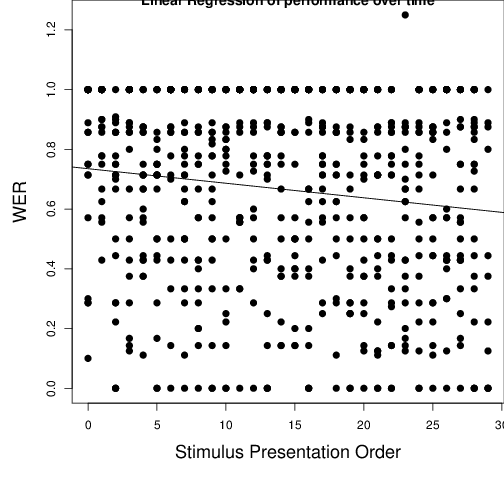
\includegraphics[width=\maxwidth]{figure/line_graph_chrono_m-1} 

\caption{Scatterplot of all participants' WER values for responses to speech recorded at the mouth \textbf{and} in noise.}
\label{fig:linear_performance_m}
\end{subfigure}
%\hfill
\begin{subfigure}{0.47\textwidth}%{L}{0.5\textwidth}

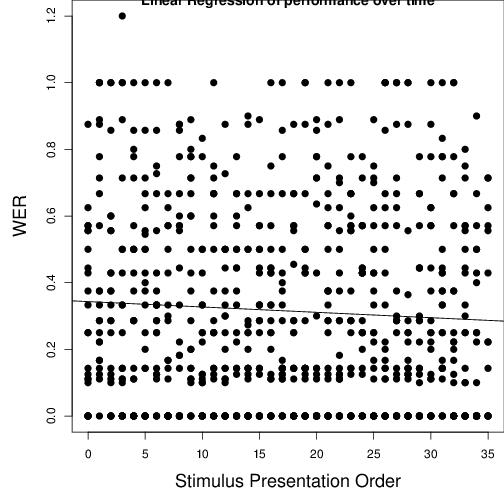
\includegraphics[width=\maxwidth]{figure/line_graph_chrono-1} 

\caption{Scatterplot of all participants' WER values for responses to speech recorded at the ear.}
\label{fig:linear_performance_e}
\end{subfigure}
\caption{The x-axis is the order of the responses; eg. `1 on the x-axis is the first response given by the participants.  The x-axis only corresponds to order of response, and does not indicate the specific noise type or gender of the speaker.  A line was fitted to the data using linear regression.}
\end{figure}
%
Linear regression models were fit onto the mouth-recorded data (slope=$-0.0048728$, $R^2$=$0.0175763$, $p<0.001$), and the ear-recorded data (slope=$-0.0016076$, $R^2$=$0.003146$, $p>0.05$). 

It is important to note the linear scales both for both axes, particularly the y-axis, as an explanation for why the slope values themselves are so small (ie. the y-axis range is from \textit{0.0} to \textit{1.2}).  The primary take away from both graphs and both fitted regression models in Figures \ref{fig:linear_performance_m} and \ref{fig:linear_performance_e} is that participants' recognition ability seems to improve statistically over the course of the experiment for mouth-recorded (noisy) speech, but not ear-recorded speech.  It could be possible that there are statistical gains by the noisy speech simply due to greater room for improvement, but it could also be due to the presence of high frequency speech information in the signal which leads to better recognition. The mouth-recorded speech beneath the noise is `normal', containing full frequency information that the participant would be accustomed to listening for, and if participants are able to use any training received to release the noise mask, this improvement over time is the expected effect.  However, as already seen, the overall performance on noisy, mouth recorded speech still falls well below that of ear-recorded speech, even at the chronological end of the experiment (cf. Figs. \ref{fig:linear_performance_m} and \ref{fig:linear_performance_e}).

%Of particular interest for the goals of this study, is the fact that - although very modest - there is improvement in recognition of ear-recorded speech that appears to correlate with an increase in exposure time to the ear-recorded speech.  That is, as more ear-recorded speech is heard, participants see modest gains in their ability to correctly recognize and transcribe it.  
One potential reason that there may not have been a statistical `training' effect for ear-recorded speech over the course of the experiment is that the participant was not given feedback or the correct answer.  It has been shown (\cite{davis:05}) that such feedback can improve and speed up the training process when listeners are able to correctly identify what was said.  This will be discussed further in Section \ref{chap3:follow-up-expts} below, and a follow up investigation will be conducted pertaining to this.


\section{Follow-up Investigations}
\label{chap3:follow-up-expts}

To expand on the previous study, two additional investigations were performed to give insights into possible future research directions.  The impetus for the first investigation was \cite{bird:97}, which demonstrated that fundamental frequency (F0) is a tool used by the auditory system to separate a desired source from masking noise.  This follow up proposed to recombine the very clear, lower frequencies from the ear-recorded speech with the `noisy' upper frequencies recorded at the mouth.  

The hypothesis was that the auditory system would use the clear fundamental frequency harmonic information in the lower frequencies to extract the upper harmonics out of the noise.  Accuracy was predicted to improve over that of the low-pass filtered, `muffled', ear speech (which many participants subjectively observed to be annoying and difficult to understand), as more high frequency information will be present and available for listeners' auditory systems.  This speech sacrificed the advantage of being completely or nearly `noise-free', to sound more natural.  Additionally, since the ear-recorded speech consisted of very clean harmonics, it was hypothesized that this speech, combined with the higher frequency mouth recorded speech in the `clean' condition, would perform equally to its mouth-recorded counterpart in the `clean' condition. This is referred to throughout as the `F0' investigation.

The second investigation was based on the concept of `training' discussed earlier.  This presumed that the auditory system can learn to adapt to understand speech in a degraded signal better with experience.  According to \cite{mattys:12}, significant learning has occurred with even a small number of training trials.  \cite{davis:05} demonstrated that during training, successful recognition of a degraded signal, more than unsuccessful recognition of a degraded signal, helped participants recognize a similar signal later on.  
Based on the implications of these findings, a short story was read aloud and recorded from inside the ear canal; this served as training for participants in a follow-up investigation.  Since the type of distortion from the ear-recorded signal was regular and predictable, it was hypothesized that those who have listened to the training story would perform better on ear-recorded speech than those who had not received training (ie. those in the primary study). This is referred to throughout as the `training' investigation.

These two investigations did not contain a full (24) number of subjects to place each participant into a counter-balanced group as these were designed as pilot studies for future research.  Therefore no statistical analysis was conducted for either investigation.  %In light of this, these could be thought of as `pilot' studies for future research.  
Because there were no individual statistical results, and because the two studies were primarily of interest when compared with the results from the primary study, the methods sections (Sections \ref{F0-methods} and \ref{training-methods}) for both studies are consecutive, and any discussion of results is withheld until Section \ref{chap3:glob_discussion}.

% for the participants in this follow-up investigation to listen to prior to completing the experiment itself. This speech will be modified in the same manner as the ear-recorded speech in the primary study (pre-emphasized, low-pass filtered 0 to 2.5 kHz with a 500 Hz slope, and pre-emphasized).  This recording did not combine the ear-recorded speech with the higher frequencies of the mouth recorded speech (as in the `F0' investigation above).  This brief story will serve as a training for participants in preparation for the actual task. 


\section{`F0' Investigation Methods}
\label{F0-methods}

\subsection{Stimuli}\label{F0-stimuli}

The stimuli used for this investigation consisted of the same 80 Harvard Sentences produced by the same speakers in the primary study above (Section \ref{expt3}).
No modification was performed to the sentences recorded at the mouth.  For the sentences recorded at the ear, the same modifications as before (pre-emphasis, low-pass filtering from 0 to 2.5 kHz with a 500 Hz slope, and a second pre-emphasis) were performed, but afterwards, the simultaneously recorded speech from the mouth was filtered and combined with the ear-recorded speech.  The speech from the mouth was bandpass filtered between 3.0 kHz and 8.0 kHz, with a 500Hz slope.  

This allowed for an overlap of the frequencies from the mouth-recorded speech and the low-pass filtered ear-recorded speech.  The two signals were converted to a stereo signal, and then combined into a mono signal.  This resulted in relatively clean speech below approximately 2.7 kHz, and noisy speech above approximately 2.7 kHz, as seen in Figure \ref{fig:combined-signal}.
%
\begin{wrapfigure}{r}{0.5\textwidth}
\centering
  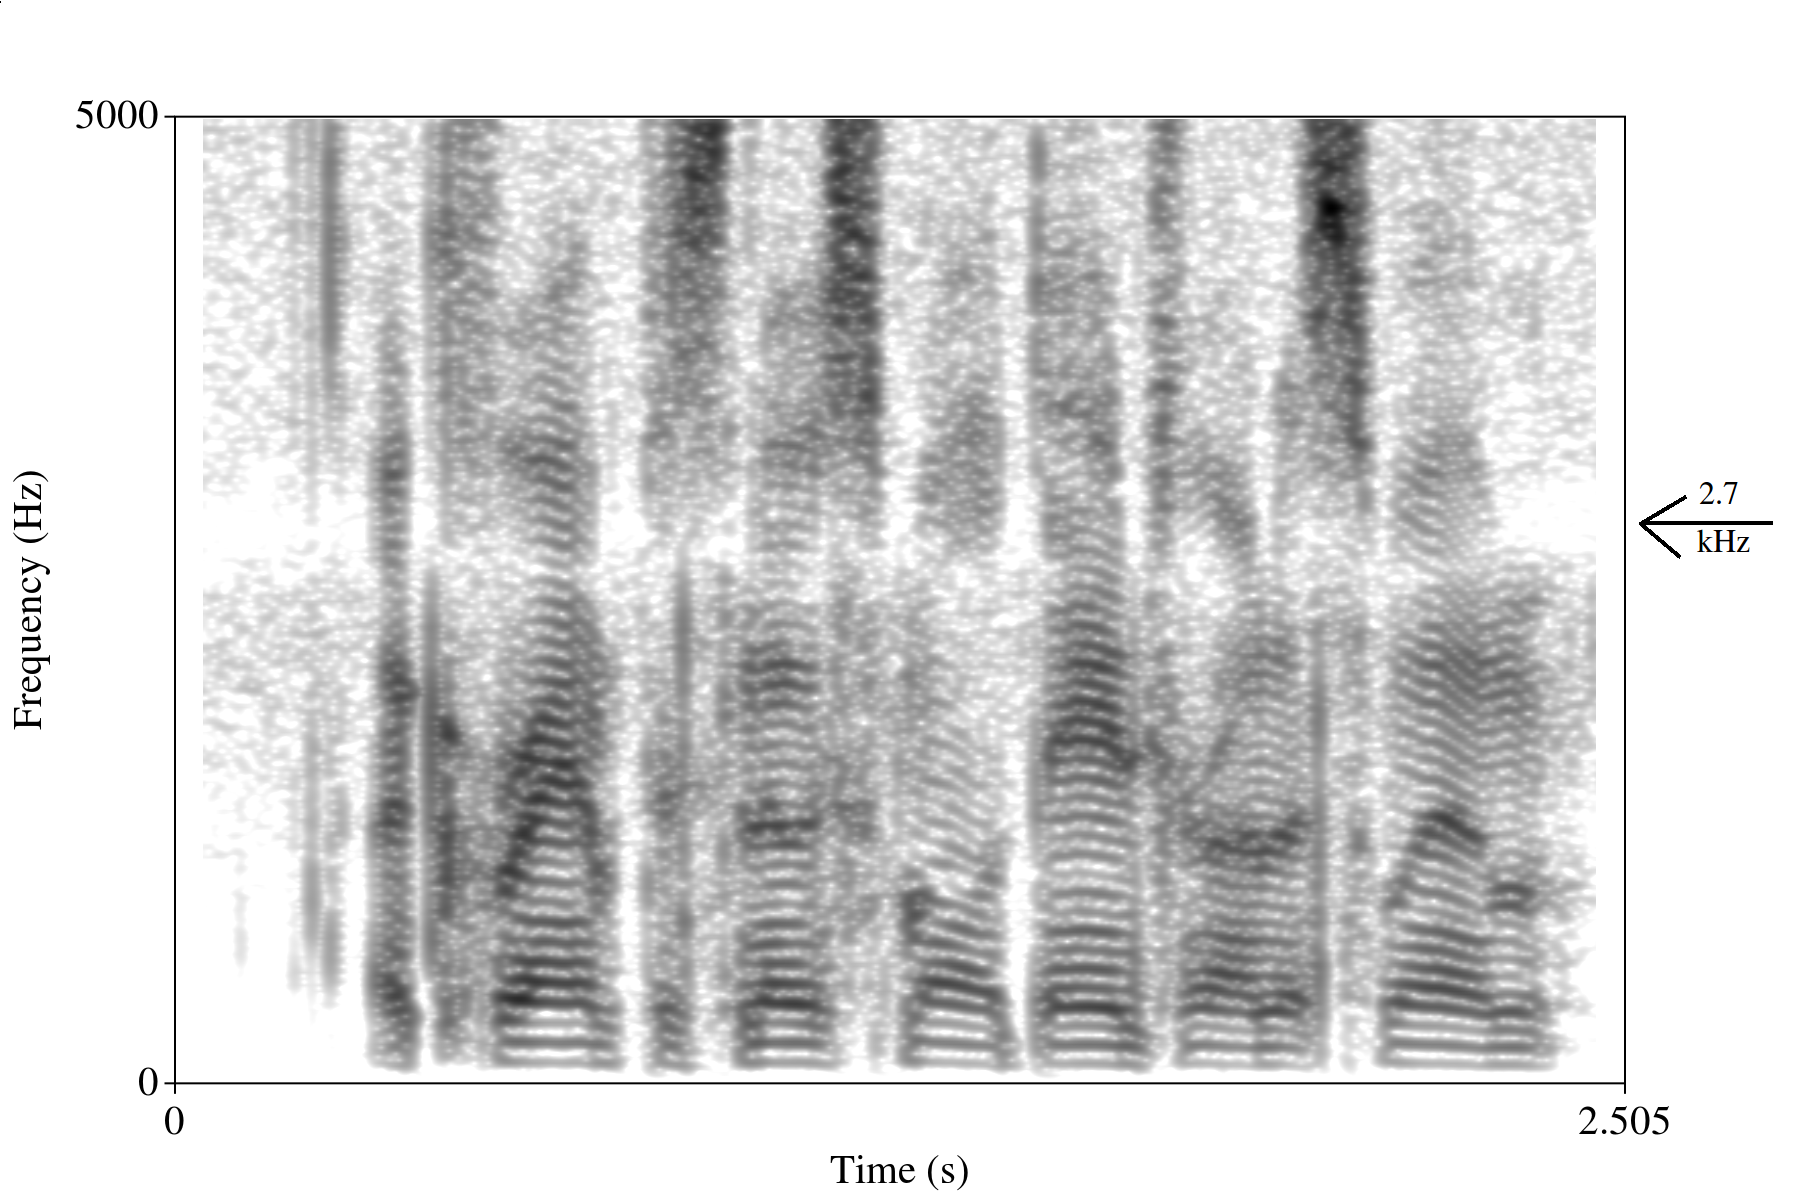
\includegraphics[width=0.45\textwidth]{figure/combined-signal_labeled.png}
  \caption{A spectrogram of the sentence ``A cramp is no small danger on a swim''.  The low-pass filtered ear-recorded signal (0 - 2.5 kHz with a 500 Hz slope) was combined with the simultaneous [noisy] mouth signal, which was bandpass filtered at a higher frequency.  The arrow indicates the location of overlap, above which the mouth-recorded signal is dominant, and below which the ear-recorded signal is dominant.}
  \label{fig:combined-signal}
\end{wrapfigure}
%

\subsection{Participants}
There were five native speakers of English with self-reported normal hearing who participated in this investigation.  

\subsection{Procedure}
The procedure of this task was exactly the same as the initial perception experiment (Section \ref{chap3:methods:procedure}), with the exception of the stimulus modification, described in Section \ref{F0-stimuli} above.


% \subsection{`F0' Results and Discussion}
% \label{chap3:F0_discussion}

%\begin{wrapfigure}{L}{0.75\textwidth}

\begin{kframe}


{\ttfamily\noindent\itshape\color{messagecolor}{\#\# The following objects are masked from mydata (pos = 3):\\\#\# \\\#\#\ \ \ \  group, mic\_location, noise\_type, sentence, sentence\_number,\\\#\#\ \ \ \  speaker\_gender, subject, wer}}

{\ttfamily\noindent\itshape\color{messagecolor}{\#\# The following objects are masked from mydata (pos = 4):\\\#\# \\\#\#\ \ \ \  group, mic\_location, noise\_type, sentence, sentence\_number,\\\#\#\ \ \ \  speaker\_gender, subject, wer}}

{\ttfamily\noindent\itshape\color{messagecolor}{\#\# The following objects are masked from mydata (pos = 5):\\\#\# \\\#\#\ \ \ \  group, mic\_location, noise\_type, sentence, sentence\_number,\\\#\#\ \ \ \  speaker\_gender, subject, wer}}

{\ttfamily\noindent\itshape\color{messagecolor}{\#\# The following objects are masked from mydata (pos = 6):\\\#\# \\\#\#\ \ \ \  group, mic\_location, noise\_type, sentence, sentence\_number,\\\#\#\ \ \ \  speaker\_gender, subject, wer}}

{\ttfamily\noindent\itshape\color{messagecolor}{\#\# The following objects are masked from mydata (pos = 7):\\\#\# \\\#\#\ \ \ \  group, mic\_location, noise\_type, sentence, sentence\_number,\\\#\#\ \ \ \  speaker\_gender, subject, wer}}

{\ttfamily\noindent\itshape\color{messagecolor}{\#\# The following objects are masked from F0data (pos = 3):\\\#\# \\\#\#\ \ \ \  group, mic\_location, noise\_type, sentence, sentence\_number,\\\#\#\ \ \ \  speaker\_gender, subject, wer}}

{\ttfamily\noindent\itshape\color{messagecolor}{\#\# The following objects are masked from mydata (pos = 4):\\\#\# \\\#\#\ \ \ \  group, mic\_location, noise\_type, sentence, sentence\_number,\\\#\#\ \ \ \  speaker\_gender, subject, wer}}

{\ttfamily\noindent\itshape\color{messagecolor}{\#\# The following objects are masked from mydata (pos = 5):\\\#\# \\\#\#\ \ \ \  group, mic\_location, noise\_type, sentence, sentence\_number,\\\#\#\ \ \ \  speaker\_gender, subject, wer}}

{\ttfamily\noindent\itshape\color{messagecolor}{\#\# The following objects are masked from mydata (pos = 6):\\\#\# \\\#\#\ \ \ \  group, mic\_location, noise\_type, sentence, sentence\_number,\\\#\#\ \ \ \  speaker\_gender, subject, wer}}

{\ttfamily\noindent\itshape\color{messagecolor}{\#\# The following objects are masked from mydata (pos = 7):\\\#\# \\\#\#\ \ \ \  group, mic\_location, noise\_type, sentence, sentence\_number,\\\#\#\ \ \ \  speaker\_gender, subject, wer}}

{\ttfamily\noindent\itshape\color{messagecolor}{\#\# The following objects are masked from mydata (pos = 8):\\\#\# \\\#\#\ \ \ \  group, mic\_location, noise\_type, sentence, sentence\_number,\\\#\#\ \ \ \  speaker\_gender, subject, wer}}

{\ttfamily\noindent\itshape\color{messagecolor}{\#\# The following objects are masked from F0data (pos = 3):\\\#\# \\\#\#\ \ \ \  group, mic\_location, noise\_type, sentence, sentence\_number,\\\#\#\ \ \ \  speaker\_gender, subject, wer}}

{\ttfamily\noindent\itshape\color{messagecolor}{\#\# The following objects are masked from F0data (pos = 4):\\\#\# \\\#\#\ \ \ \  group, mic\_location, noise\_type, sentence, sentence\_number,\\\#\#\ \ \ \  speaker\_gender, subject, wer}}

{\ttfamily\noindent\itshape\color{messagecolor}{\#\# The following objects are masked from mydata (pos = 5):\\\#\# \\\#\#\ \ \ \  group, mic\_location, noise\_type, sentence, sentence\_number,\\\#\#\ \ \ \  speaker\_gender, subject, wer}}

{\ttfamily\noindent\itshape\color{messagecolor}{\#\# The following objects are masked from mydata (pos = 6):\\\#\# \\\#\#\ \ \ \  group, mic\_location, noise\_type, sentence, sentence\_number,\\\#\#\ \ \ \  speaker\_gender, subject, wer}}

{\ttfamily\noindent\itshape\color{messagecolor}{\#\# The following objects are masked from mydata (pos = 7):\\\#\# \\\#\#\ \ \ \  group, mic\_location, noise\_type, sentence, sentence\_number,\\\#\#\ \ \ \  speaker\_gender, subject, wer}}

{\ttfamily\noindent\itshape\color{messagecolor}{\#\# The following objects are masked from mydata (pos = 8):\\\#\# \\\#\#\ \ \ \  group, mic\_location, noise\_type, sentence, sentence\_number,\\\#\#\ \ \ \  speaker\_gender, subject, wer}}

{\ttfamily\noindent\itshape\color{messagecolor}{\#\# The following objects are masked from mydata (pos = 9):\\\#\# \\\#\#\ \ \ \  group, mic\_location, noise\_type, sentence, sentence\_number,\\\#\#\ \ \ \  speaker\_gender, subject, wer}}

{\ttfamily\noindent\itshape\color{messagecolor}{\#\# The following objects are masked from F0data (pos = 3):\\\#\# \\\#\#\ \ \ \  group, mic\_location, noise\_type, sentence, sentence\_number,\\\#\#\ \ \ \  speaker\_gender, subject, wer}}

{\ttfamily\noindent\itshape\color{messagecolor}{\#\# The following objects are masked from F0data (pos = 4):\\\#\# \\\#\#\ \ \ \  group, mic\_location, noise\_type, sentence, sentence\_number,\\\#\#\ \ \ \  speaker\_gender, subject, wer}}

{\ttfamily\noindent\itshape\color{messagecolor}{\#\# The following objects are masked from F0data (pos = 5):\\\#\# \\\#\#\ \ \ \  group, mic\_location, noise\_type, sentence, sentence\_number,\\\#\#\ \ \ \  speaker\_gender, subject, wer}}

{\ttfamily\noindent\itshape\color{messagecolor}{\#\# The following objects are masked from mydata (pos = 6):\\\#\# \\\#\#\ \ \ \  group, mic\_location, noise\_type, sentence, sentence\_number,\\\#\#\ \ \ \  speaker\_gender, subject, wer}}

{\ttfamily\noindent\itshape\color{messagecolor}{\#\# The following objects are masked from mydata (pos = 7):\\\#\# \\\#\#\ \ \ \  group, mic\_location, noise\_type, sentence, sentence\_number,\\\#\#\ \ \ \  speaker\_gender, subject, wer}}

{\ttfamily\noindent\itshape\color{messagecolor}{\#\# The following objects are masked from mydata (pos = 8):\\\#\# \\\#\#\ \ \ \  group, mic\_location, noise\_type, sentence, sentence\_number,\\\#\#\ \ \ \  speaker\_gender, subject, wer}}

{\ttfamily\noindent\itshape\color{messagecolor}{\#\# The following objects are masked from mydata (pos = 9):\\\#\# \\\#\#\ \ \ \  group, mic\_location, noise\_type, sentence, sentence\_number,\\\#\#\ \ \ \  speaker\_gender, subject, wer}}

{\ttfamily\noindent\itshape\color{messagecolor}{\#\# The following objects are masked from mydata (pos = 10):\\\#\# \\\#\#\ \ \ \  group, mic\_location, noise\_type, sentence, sentence\_number,\\\#\#\ \ \ \  speaker\_gender, subject, wer}}

{\ttfamily\noindent\itshape\color{messagecolor}{\#\# The following objects are masked from F0data (pos = 3):\\\#\# \\\#\#\ \ \ \  group, mic\_location, noise\_type, sentence, sentence\_number,\\\#\#\ \ \ \  speaker\_gender, subject, wer}}

{\ttfamily\noindent\itshape\color{messagecolor}{\#\# The following objects are masked from F0data (pos = 4):\\\#\# \\\#\#\ \ \ \  group, mic\_location, noise\_type, sentence, sentence\_number,\\\#\#\ \ \ \  speaker\_gender, subject, wer}}

{\ttfamily\noindent\itshape\color{messagecolor}{\#\# The following objects are masked from F0data (pos = 5):\\\#\# \\\#\#\ \ \ \  group, mic\_location, noise\_type, sentence, sentence\_number,\\\#\#\ \ \ \  speaker\_gender, subject, wer}}

{\ttfamily\noindent\itshape\color{messagecolor}{\#\# The following objects are masked from F0data (pos = 6):\\\#\# \\\#\#\ \ \ \  group, mic\_location, noise\_type, sentence, sentence\_number,\\\#\#\ \ \ \  speaker\_gender, subject, wer}}

{\ttfamily\noindent\itshape\color{messagecolor}{\#\# The following objects are masked from mydata (pos = 7):\\\#\# \\\#\#\ \ \ \  group, mic\_location, noise\_type, sentence, sentence\_number,\\\#\#\ \ \ \  speaker\_gender, subject, wer}}

{\ttfamily\noindent\itshape\color{messagecolor}{\#\# The following objects are masked from mydata (pos = 8):\\\#\# \\\#\#\ \ \ \  group, mic\_location, noise\_type, sentence, sentence\_number,\\\#\#\ \ \ \  speaker\_gender, subject, wer}}

{\ttfamily\noindent\itshape\color{messagecolor}{\#\# The following objects are masked from mydata (pos = 9):\\\#\# \\\#\#\ \ \ \  group, mic\_location, noise\_type, sentence, sentence\_number,\\\#\#\ \ \ \  speaker\_gender, subject, wer}}

{\ttfamily\noindent\itshape\color{messagecolor}{\#\# The following objects are masked from mydata (pos = 10):\\\#\# \\\#\#\ \ \ \  group, mic\_location, noise\_type, sentence, sentence\_number,\\\#\#\ \ \ \  speaker\_gender, subject, wer}}

{\ttfamily\noindent\itshape\color{messagecolor}{\#\# The following objects are masked from mydata (pos = 11):\\\#\# \\\#\#\ \ \ \  group, mic\_location, noise\_type, sentence, sentence\_number,\\\#\#\ \ \ \  speaker\_gender, subject, wer}}\end{kframe}

% \caption{Using the data from the five participants who performed the experiment using the speech in which the higher frequencies were added back in from the noisy mouth-recorded speech.  Boxplot displaying the average word error rate (WER) averaged over each participant for every noise type. WER is the variable on the y-axis, and noise type is on the x-axis.}
% \label{fig:F0_noise_boxplot}
% \end{wrapfigure}

% \begin{figure}%{L}{\textwidth}
% <<F0_boxplot_noiseXspkr, echo=FALSE, results='asis'>>=
% boxplot(wer~noise_type*speaker_gender,col=c("white","lightgray"),F0data, names=c("Female\nNo Noise","Female\nBus","Female\nCafe","Female\nPedestrian","Female\nStreet","Female\nFactory","Male\nNo Noise","Male\nBus","Male\nCafe","Male\nPedestrian","Male\nStreet","Male\nFactory"),ylab="WER",las=2)
% @
% \caption{Using the data from the five participants who performed the experiment using the speech in which the higher frequencies were added back in from the noisy mouth-recorded speech.  Boxplot displaying the average word error rate (WER) averaged over each participant for the interaction of every noise type by the speaker gender. WER is the variable on the y-axis, and noise type by speaker gender is on the x-axis.}
% \label{fig:F0_noiseXspkr_boxplot}
% \end{figure}

% \begin{figure}[h!]%{L}{\textwidth}
% <<F0_boxplot_noiseXmic, echo=FALSE, results='asis'>>=
% par(mar=c(6,4,0,0))
% boxplot(wer~noise_type*mic_location,col=c("white","lightgray"),F0data, names=c("Ear\nNo Noise","Ear\nBus","Ear\nCafe","Ear\nPedestrian","Ear\nStreet","Ear\nFactory","Mouth\nNo Noise","Mouth\nBus","Mouth\nCafe","Mouth\nPedestrian","Mouth\nStreet","Mouth\nFactory"),ylab="WER",las=2)
% @
% \caption{Using the data from the five participants who performed the task using the speech in which the higher frequencies were added back in from the noisy mouth-recorded speech.  Boxplot displaying the average word error rate (WER) averaged over each participant for the interaction of every noise type by the mic location. WER is the variable on the y-axis, and noise type by mic location is on the x-axis.}
% \label{fig:F0_noiseXmic_boxplot}
% \end{figure}
% 
% Since there were only five participants in this follow-up investigation, no actual statistics were run to test for significance.  The results here are to be used in a basic comparison of possible directions these altered methods may be able to take future research.
% 
% The boxplot in Figure \ref{fig:F0_noiseXmic_boxplot} demonstrates the interaction of most interest, that of noise-type and microphone location, as identified by the ANOVAs performed on the primary experiment above.  No change was made to any of the presented mouth-recorded speech signals, so, as is observed, one would not expect there to be any change to listeners' ability to recognize these signals (outside of expected inter-speaker variation).
% 
% It is interesting to note that the primary difference between the clean ear-recorded speech and the `noisy' ear-recorded speech appears to be the extent of the variation in the upper quartile and whiskers.  Based on what is seen here, if this follow up study were to be extended carried out in a full study, one would expect there to be a dramatic difference between the noisy speech recorded at the mouth, and the speech recorded at the ear.
% Further discussion concerning the comparison of these results with those of the primary study and the `training' study can be found below in Section \ref{chap3:glob_discussion}.
% %
% \begin{wrapfigure}{L}{0.5\textwidth}
% <<F0spkr-gender_mic-location_interaction, echo=FALSE, results='asis'>>=
% boxplot(wer~speaker_gender*mic_location,col=c("white","lightgray"),F0data, names=c("Female\nEar-Recorded","Female\nMouth-Recorded","Male\nEar-Recorded","Male\nMouth-Recorded"),ylab="WER")
% @
% \caption{Interaction between speaker gender and microphone location.}
% \label{fig:F0_spkr-genXmic-loc}
% \end{wrapfigure}
% %


\section{`Training' Investigation Methods}
\label{training-methods}

\subsection{Stimuli}

The exact same stimuli from the primary experiment were used in this study. No modification was made to the speech signals, such as the one used for the `F0' investigation explained in Section \ref{F0-methods} above.

\subsection{Participants}

There were four native speakers of English with self-reported normal hearing who participated in this follow up investigation.

\subsection{Design}

This investigation aimed to test if `training' the participants on ear-recorded speech prior to the experiment resulted in an improvement in recognition during the experiment.  The training used is a `read-along' short story - `Peter Rabbit', by Beatrix Potter.  To obtain a recording of the story, a new speaker was recorded from the ear canal (using the same experimental set-up as described in Sections \ref{chap2:methods:procedure} and \ref{chap3:methods:procedure}).  No microphone was needed to record the speech from the mouth, and there was no background noise emitted during the recording.  

The recorded story, as was presented to the participants, had a total length of approximately 5 minutes and 13 seconds.  The recorded story underwent the same transformations as the ear-recorded stimuli in the primary study (ie. pre-emphasis, low-pass filtering\footnote{low-pass filter of 0-2500Hz with a 500Hz slope.}, and pre-emphasis again).  The participants would be presented with a typed transcript of the story with which to follow along.  This provided real-time recognition feedback and offered ample chance for `successful' recognition of the degraded ear-recorded signal (cf. \cite{davis:05}).

\subsection{Procedure}

The participants entered the sound booth and were presented with a transcript of the short story and were asked to listen to the audio (ear-recorded narration) and read along.  After the `training' session, the participants conducted the task as was done in the other studies (cf. Sections \ref{chap3:methods:procedure} and \ref{F0-methods}).

% \subsection{`Training' Results and Discussion}


\begin{kframe}


{\ttfamily\noindent\itshape\color{messagecolor}{\#\# The following objects are masked from F0data (pos = 3):\\\#\# \\\#\#\ \ \ \  group, mic\_location, noise\_type, sentence, sentence\_number,\\\#\#\ \ \ \  speaker\_gender, subject, wer}}

{\ttfamily\noindent\itshape\color{messagecolor}{\#\# The following objects are masked from F0data (pos = 4):\\\#\# \\\#\#\ \ \ \  group, mic\_location, noise\_type, sentence, sentence\_number,\\\#\#\ \ \ \  speaker\_gender, subject, wer}}

{\ttfamily\noindent\itshape\color{messagecolor}{\#\# The following objects are masked from F0data (pos = 5):\\\#\# \\\#\#\ \ \ \  group, mic\_location, noise\_type, sentence, sentence\_number,\\\#\#\ \ \ \  speaker\_gender, subject, wer}}

{\ttfamily\noindent\itshape\color{messagecolor}{\#\# The following objects are masked from F0data (pos = 6):\\\#\# \\\#\#\ \ \ \  group, mic\_location, noise\_type, sentence, sentence\_number,\\\#\#\ \ \ \  speaker\_gender, subject, wer}}

{\ttfamily\noindent\itshape\color{messagecolor}{\#\# The following objects are masked from F0data (pos = 7):\\\#\# \\\#\#\ \ \ \  group, mic\_location, noise\_type, sentence, sentence\_number,\\\#\#\ \ \ \  speaker\_gender, subject, wer}}

{\ttfamily\noindent\itshape\color{messagecolor}{\#\# The following objects are masked from mydata (pos = 8):\\\#\# \\\#\#\ \ \ \  group, mic\_location, noise\_type, sentence, sentence\_number,\\\#\#\ \ \ \  speaker\_gender, subject, wer}}

{\ttfamily\noindent\itshape\color{messagecolor}{\#\# The following objects are masked from mydata (pos = 9):\\\#\# \\\#\#\ \ \ \  group, mic\_location, noise\_type, sentence, sentence\_number,\\\#\#\ \ \ \  speaker\_gender, subject, wer}}

{\ttfamily\noindent\itshape\color{messagecolor}{\#\# The following objects are masked from mydata (pos = 10):\\\#\# \\\#\#\ \ \ \  group, mic\_location, noise\_type, sentence, sentence\_number,\\\#\#\ \ \ \  speaker\_gender, subject, wer}}

{\ttfamily\noindent\itshape\color{messagecolor}{\#\# The following objects are masked from mydata (pos = 11):\\\#\# \\\#\#\ \ \ \  group, mic\_location, noise\_type, sentence, sentence\_number,\\\#\#\ \ \ \  speaker\_gender, subject, wer}}

{\ttfamily\noindent\itshape\color{messagecolor}{\#\# The following objects are masked from mydata (pos = 12):\\\#\# \\\#\#\ \ \ \  group, mic\_location, noise\_type, sentence, sentence\_number,\\\#\#\ \ \ \  speaker\_gender, subject, wer}}

{\ttfamily\noindent\itshape\color{messagecolor}{\#\# The following objects are masked from perc\_data (pos = 3):\\\#\# \\\#\#\ \ \ \  group, mic\_location, noise\_type, sentence, sentence\_number,\\\#\#\ \ \ \  speaker\_gender, subject, wer}}

{\ttfamily\noindent\itshape\color{messagecolor}{\#\# The following objects are masked from F0data (pos = 4):\\\#\# \\\#\#\ \ \ \  group, mic\_location, noise\_type, sentence, sentence\_number,\\\#\#\ \ \ \  speaker\_gender, subject, wer}}

{\ttfamily\noindent\itshape\color{messagecolor}{\#\# The following objects are masked from F0data (pos = 5):\\\#\# \\\#\#\ \ \ \  group, mic\_location, noise\_type, sentence, sentence\_number,\\\#\#\ \ \ \  speaker\_gender, subject, wer}}

{\ttfamily\noindent\itshape\color{messagecolor}{\#\# The following objects are masked from F0data (pos = 6):\\\#\# \\\#\#\ \ \ \  group, mic\_location, noise\_type, sentence, sentence\_number,\\\#\#\ \ \ \  speaker\_gender, subject, wer}}

{\ttfamily\noindent\itshape\color{messagecolor}{\#\# The following objects are masked from F0data (pos = 7):\\\#\# \\\#\#\ \ \ \  group, mic\_location, noise\_type, sentence, sentence\_number,\\\#\#\ \ \ \  speaker\_gender, subject, wer}}

{\ttfamily\noindent\itshape\color{messagecolor}{\#\# The following objects are masked from F0data (pos = 8):\\\#\# \\\#\#\ \ \ \  group, mic\_location, noise\_type, sentence, sentence\_number,\\\#\#\ \ \ \  speaker\_gender, subject, wer}}

{\ttfamily\noindent\itshape\color{messagecolor}{\#\# The following objects are masked from mydata (pos = 9):\\\#\# \\\#\#\ \ \ \  group, mic\_location, noise\_type, sentence, sentence\_number,\\\#\#\ \ \ \  speaker\_gender, subject, wer}}

{\ttfamily\noindent\itshape\color{messagecolor}{\#\# The following objects are masked from mydata (pos = 10):\\\#\# \\\#\#\ \ \ \  group, mic\_location, noise\_type, sentence, sentence\_number,\\\#\#\ \ \ \  speaker\_gender, subject, wer}}

{\ttfamily\noindent\itshape\color{messagecolor}{\#\# The following objects are masked from mydata (pos = 11):\\\#\# \\\#\#\ \ \ \  group, mic\_location, noise\_type, sentence, sentence\_number,\\\#\#\ \ \ \  speaker\_gender, subject, wer}}

{\ttfamily\noindent\itshape\color{messagecolor}{\#\# The following objects are masked from mydata (pos = 12):\\\#\# \\\#\#\ \ \ \  group, mic\_location, noise\_type, sentence, sentence\_number,\\\#\#\ \ \ \  speaker\_gender, subject, wer}}

{\ttfamily\noindent\itshape\color{messagecolor}{\#\# The following objects are masked from mydata (pos = 13):\\\#\# \\\#\#\ \ \ \  group, mic\_location, noise\_type, sentence, sentence\_number,\\\#\#\ \ \ \  speaker\_gender, subject, wer}}

{\ttfamily\noindent\itshape\color{messagecolor}{\#\# The following objects are masked from perc\_data (pos = 3):\\\#\# \\\#\#\ \ \ \  group, mic\_location, noise\_type, sentence, sentence\_number,\\\#\#\ \ \ \  speaker\_gender, subject, wer}}

{\ttfamily\noindent\itshape\color{messagecolor}{\#\# The following objects are masked from perc\_data (pos = 4):\\\#\# \\\#\#\ \ \ \  group, mic\_location, noise\_type, sentence, sentence\_number,\\\#\#\ \ \ \  speaker\_gender, subject, wer}}

{\ttfamily\noindent\itshape\color{messagecolor}{\#\# The following objects are masked from F0data (pos = 5):\\\#\# \\\#\#\ \ \ \  group, mic\_location, noise\_type, sentence, sentence\_number,\\\#\#\ \ \ \  speaker\_gender, subject, wer}}

{\ttfamily\noindent\itshape\color{messagecolor}{\#\# The following objects are masked from F0data (pos = 6):\\\#\# \\\#\#\ \ \ \  group, mic\_location, noise\_type, sentence, sentence\_number,\\\#\#\ \ \ \  speaker\_gender, subject, wer}}

{\ttfamily\noindent\itshape\color{messagecolor}{\#\# The following objects are masked from F0data (pos = 7):\\\#\# \\\#\#\ \ \ \  group, mic\_location, noise\_type, sentence, sentence\_number,\\\#\#\ \ \ \  speaker\_gender, subject, wer}}

{\ttfamily\noindent\itshape\color{messagecolor}{\#\# The following objects are masked from F0data (pos = 8):\\\#\# \\\#\#\ \ \ \  group, mic\_location, noise\_type, sentence, sentence\_number,\\\#\#\ \ \ \  speaker\_gender, subject, wer}}

{\ttfamily\noindent\itshape\color{messagecolor}{\#\# The following objects are masked from F0data (pos = 9):\\\#\# \\\#\#\ \ \ \  group, mic\_location, noise\_type, sentence, sentence\_number,\\\#\#\ \ \ \  speaker\_gender, subject, wer}}

{\ttfamily\noindent\itshape\color{messagecolor}{\#\# The following objects are masked from mydata (pos = 10):\\\#\# \\\#\#\ \ \ \  group, mic\_location, noise\_type, sentence, sentence\_number,\\\#\#\ \ \ \  speaker\_gender, subject, wer}}

{\ttfamily\noindent\itshape\color{messagecolor}{\#\# The following objects are masked from mydata (pos = 11):\\\#\# \\\#\#\ \ \ \  group, mic\_location, noise\_type, sentence, sentence\_number,\\\#\#\ \ \ \  speaker\_gender, subject, wer}}

{\ttfamily\noindent\itshape\color{messagecolor}{\#\# The following objects are masked from mydata (pos = 12):\\\#\# \\\#\#\ \ \ \  group, mic\_location, noise\_type, sentence, sentence\_number,\\\#\#\ \ \ \  speaker\_gender, subject, wer}}

{\ttfamily\noindent\itshape\color{messagecolor}{\#\# The following objects are masked from mydata (pos = 13):\\\#\# \\\#\#\ \ \ \  group, mic\_location, noise\_type, sentence, sentence\_number,\\\#\#\ \ \ \  speaker\_gender, subject, wer}}

{\ttfamily\noindent\itshape\color{messagecolor}{\#\# The following objects are masked from mydata (pos = 14):\\\#\# \\\#\#\ \ \ \  group, mic\_location, noise\_type, sentence, sentence\_number,\\\#\#\ \ \ \  speaker\_gender, subject, wer}}

{\ttfamily\noindent\itshape\color{messagecolor}{\#\# The following objects are masked from perc\_data (pos = 3):\\\#\# \\\#\#\ \ \ \  group, mic\_location, noise\_type, sentence, sentence\_number,\\\#\#\ \ \ \  speaker\_gender, subject, wer}}

{\ttfamily\noindent\itshape\color{messagecolor}{\#\# The following objects are masked from perc\_data (pos = 4):\\\#\# \\\#\#\ \ \ \  group, mic\_location, noise\_type, sentence, sentence\_number,\\\#\#\ \ \ \  speaker\_gender, subject, wer}}

{\ttfamily\noindent\itshape\color{messagecolor}{\#\# The following objects are masked from perc\_data (pos = 5):\\\#\# \\\#\#\ \ \ \  group, mic\_location, noise\_type, sentence, sentence\_number,\\\#\#\ \ \ \  speaker\_gender, subject, wer}}

{\ttfamily\noindent\itshape\color{messagecolor}{\#\# The following objects are masked from F0data (pos = 6):\\\#\# \\\#\#\ \ \ \  group, mic\_location, noise\_type, sentence, sentence\_number,\\\#\#\ \ \ \  speaker\_gender, subject, wer}}

{\ttfamily\noindent\itshape\color{messagecolor}{\#\# The following objects are masked from F0data (pos = 7):\\\#\# \\\#\#\ \ \ \  group, mic\_location, noise\_type, sentence, sentence\_number,\\\#\#\ \ \ \  speaker\_gender, subject, wer}}

{\ttfamily\noindent\itshape\color{messagecolor}{\#\# The following objects are masked from F0data (pos = 8):\\\#\# \\\#\#\ \ \ \  group, mic\_location, noise\_type, sentence, sentence\_number,\\\#\#\ \ \ \  speaker\_gender, subject, wer}}

{\ttfamily\noindent\itshape\color{messagecolor}{\#\# The following objects are masked from F0data (pos = 9):\\\#\# \\\#\#\ \ \ \  group, mic\_location, noise\_type, sentence, sentence\_number,\\\#\#\ \ \ \  speaker\_gender, subject, wer}}

{\ttfamily\noindent\itshape\color{messagecolor}{\#\# The following objects are masked from F0data (pos = 10):\\\#\# \\\#\#\ \ \ \  group, mic\_location, noise\_type, sentence, sentence\_number,\\\#\#\ \ \ \  speaker\_gender, subject, wer}}

{\ttfamily\noindent\itshape\color{messagecolor}{\#\# The following objects are masked from mydata (pos = 11):\\\#\# \\\#\#\ \ \ \  group, mic\_location, noise\_type, sentence, sentence\_number,\\\#\#\ \ \ \  speaker\_gender, subject, wer}}

{\ttfamily\noindent\itshape\color{messagecolor}{\#\# The following objects are masked from mydata (pos = 12):\\\#\# \\\#\#\ \ \ \  group, mic\_location, noise\_type, sentence, sentence\_number,\\\#\#\ \ \ \  speaker\_gender, subject, wer}}

{\ttfamily\noindent\itshape\color{messagecolor}{\#\# The following objects are masked from mydata (pos = 13):\\\#\# \\\#\#\ \ \ \  group, mic\_location, noise\_type, sentence, sentence\_number,\\\#\#\ \ \ \  speaker\_gender, subject, wer}}

{\ttfamily\noindent\itshape\color{messagecolor}{\#\# The following objects are masked from mydata (pos = 14):\\\#\# \\\#\#\ \ \ \  group, mic\_location, noise\_type, sentence, sentence\_number,\\\#\#\ \ \ \  speaker\_gender, subject, wer}}

{\ttfamily\noindent\itshape\color{messagecolor}{\#\# The following objects are masked from mydata (pos = 15):\\\#\# \\\#\#\ \ \ \  group, mic\_location, noise\_type, sentence, sentence\_number,\\\#\#\ \ \ \  speaker\_gender, subject, wer}}

{\ttfamily\noindent\itshape\color{messagecolor}{\#\# The following objects are masked from perc\_data (pos = 3):\\\#\# \\\#\#\ \ \ \  group, mic\_location, noise\_type, sentence, sentence\_number,\\\#\#\ \ \ \  speaker\_gender, subject, wer}}

{\ttfamily\noindent\itshape\color{messagecolor}{\#\# The following objects are masked from perc\_data (pos = 4):\\\#\# \\\#\#\ \ \ \  group, mic\_location, noise\_type, sentence, sentence\_number,\\\#\#\ \ \ \  speaker\_gender, subject, wer}}

{\ttfamily\noindent\itshape\color{messagecolor}{\#\# The following objects are masked from perc\_data (pos = 5):\\\#\# \\\#\#\ \ \ \  group, mic\_location, noise\_type, sentence, sentence\_number,\\\#\#\ \ \ \  speaker\_gender, subject, wer}}

{\ttfamily\noindent\itshape\color{messagecolor}{\#\# The following objects are masked from perc\_data (pos = 6):\\\#\# \\\#\#\ \ \ \  group, mic\_location, noise\_type, sentence, sentence\_number,\\\#\#\ \ \ \  speaker\_gender, subject, wer}}

{\ttfamily\noindent\itshape\color{messagecolor}{\#\# The following objects are masked from F0data (pos = 7):\\\#\# \\\#\#\ \ \ \  group, mic\_location, noise\_type, sentence, sentence\_number,\\\#\#\ \ \ \  speaker\_gender, subject, wer}}

{\ttfamily\noindent\itshape\color{messagecolor}{\#\# The following objects are masked from F0data (pos = 8):\\\#\# \\\#\#\ \ \ \  group, mic\_location, noise\_type, sentence, sentence\_number,\\\#\#\ \ \ \  speaker\_gender, subject, wer}}

{\ttfamily\noindent\itshape\color{messagecolor}{\#\# The following objects are masked from F0data (pos = 9):\\\#\# \\\#\#\ \ \ \  group, mic\_location, noise\_type, sentence, sentence\_number,\\\#\#\ \ \ \  speaker\_gender, subject, wer}}

{\ttfamily\noindent\itshape\color{messagecolor}{\#\# The following objects are masked from F0data (pos = 10):\\\#\# \\\#\#\ \ \ \  group, mic\_location, noise\_type, sentence, sentence\_number,\\\#\#\ \ \ \  speaker\_gender, subject, wer}}

{\ttfamily\noindent\itshape\color{messagecolor}{\#\# The following objects are masked from F0data (pos = 11):\\\#\# \\\#\#\ \ \ \  group, mic\_location, noise\_type, sentence, sentence\_number,\\\#\#\ \ \ \  speaker\_gender, subject, wer}}

{\ttfamily\noindent\itshape\color{messagecolor}{\#\# The following objects are masked from mydata (pos = 12):\\\#\# \\\#\#\ \ \ \  group, mic\_location, noise\_type, sentence, sentence\_number,\\\#\#\ \ \ \  speaker\_gender, subject, wer}}

{\ttfamily\noindent\itshape\color{messagecolor}{\#\# The following objects are masked from mydata (pos = 13):\\\#\# \\\#\#\ \ \ \  group, mic\_location, noise\_type, sentence, sentence\_number,\\\#\#\ \ \ \  speaker\_gender, subject, wer}}

{\ttfamily\noindent\itshape\color{messagecolor}{\#\# The following objects are masked from mydata (pos = 14):\\\#\# \\\#\#\ \ \ \  group, mic\_location, noise\_type, sentence, sentence\_number,\\\#\#\ \ \ \  speaker\_gender, subject, wer}}

{\ttfamily\noindent\itshape\color{messagecolor}{\#\# The following objects are masked from mydata (pos = 15):\\\#\# \\\#\#\ \ \ \  group, mic\_location, noise\_type, sentence, sentence\_number,\\\#\#\ \ \ \  speaker\_gender, subject, wer}}

{\ttfamily\noindent\itshape\color{messagecolor}{\#\# The following objects are masked from mydata (pos = 16):\\\#\# \\\#\#\ \ \ \  group, mic\_location, noise\_type, sentence, sentence\_number,\\\#\#\ \ \ \  speaker\_gender, subject, wer}}\end{kframe}

% \caption{Using the data from the four participants who performed the training task in which they listened and read along to a story prior to the experiment.  Boxplot displaying the average word error rate (WER) averaged over each participant for every noise type. WER is the variable on the y-axis, and noise type is on the x-axis.}
% \label{fig:perc_noise_boxplot}
% \end{wrapfigure}

% \begin{wrapfigure}{L}{\textwidth}
% <<perc_boxplot_noiseXspkr, echo=FALSE, results='asis'>>=
% boxplot(wer~noise_type*speaker_gender,col=c("white","lightgray"),perc_data, names=c("Female\nNo Noise","Female\nBus","Female\nCafe","Female\nPedestrian","Female\nStreet","Female\nFactory","Male\nNo Noise","Male\nBus","Male\nCafe","Male\nPedestrian","Male\nStreet","Male\nFactory"),ylab="WER",las=2)
% @
% \caption{Using the data from the four participants who performed the training task in which they listened and read along to a story prior to the experiment.  Boxplot displaying the average word error rate (WER) averaged over each participant for the interaction of every noise type by the speaker gender. WER is the variable on the y-axis, and noise type by speaker gender is on the x-axis.}
% \label{fig:perc_noiseXspkr_boxplot}
% \end{wrapfigure}

% \begin{figure}[h!]
% <<perc_boxplot_noiseXmic, echo=FALSE, results='asis'>>=
% par(mar=c(6,4,0,0))
% boxplot(wer~noise_type*mic_location,col=c("white","lightgray"),perc_data, names=c("Ear\nNo Noise","Ear\nBus","Ear\nCafe","Ear\nPedestrian","Ear\nStreet","Ear\nFactory","Mouth\nNo Noise","Mouth\nBus","Mouth\nCafe","Mouth\nPedestrian","Mouth\nStreet","Mouth\nFactory"),ylab="WER",las=2)
% @
% \caption{Using the data from the four participants who performed the training task in which they listened and read along to a story prior to the experiment. Boxplot displaying the average word error rate (WER) averaged over each participant for the interaction of every noise type by the mic location. WER is the variable on the y-axis, and noise type by mic location is on the x-axis.}
% \label{fig:perc_noiseXmic_boxplot}
% \end{figure}
% 
% As stated in the discussion of the `F0' investigation in Section \ref{chap3:F0_discussion}, there are too few participants to run actual statistics on the results of this follow up investigation, and so implications here should be taken lightly and used to prepare further future research in this area. The only difference between this investigation and the primary study are that the participants in this task heard a 5 minute, 13 second `training' story beforehand, recorded from the story narrator's ear.
% 
% The boxplot in Figure \ref{fig:perc_noiseXmic_boxplot} displays the interaction of noise type and microphone location, which was a statistical interaction in the primary experiment.  It can be seen that the relationship between ear- and noisy mouth-recorded speech appear to remain the same; as expected the ear-recorded speech continues to be more easily recognized than speech recorded at the mouth in noise.  Further discussion continues below.



\subsection{Discussion of All Investigations}
\label{chap3:glob_discussion}

Looking into the differences between the primary study and the two follow-up studies, Figures \ref{fig:female-all} and \ref{fig:male-all} split the results by gender into female-speaker and male-speaker data, respectively.  Given that no change was actually made to the audio of the mouth-recorded speech between these different experiments, there is expected to be no substantial observable difference between the three studies, in each condition, which is largely what is seen.  There is, of course, variation among the WERs on mouth-recorded signals, but this is not expected to be significant if tested statistically.  It is possible that the study involving the training task, exposing listeners to degraded speech, would help `train' their auditory system to be more perceptive overall, but this is not expected to result in significant benefit.




\begin{figure}[h!]

\includegraphics[width=\maxwidth]{figure/boxplot_noiseXmicXall_female-1} 

\caption{Boxplot displaying the average word error rate (WER) averaged over each participant for the interaction of every noise type by the mic location, for all three studies; this is data for only recognition on utterances by the female speaker. WER is the variable on the y-axis, and noise type by mic location is on the x-axis. (`P',gray,`Primary' study); (`F0',green,`F0' study); (`T',blue,`Training' study); (`E',lighter color,`Ear-recorded'); (`M',darker color,`Mouth-recorded'). `EH' = Ear-recorded with reintroduction of high frequencies (from mouth-recorded speech).}
\label{fig:female-all}
\end{figure}

\begin{figure}[h!]

\includegraphics[width=\maxwidth]{figure/boxplot_noiseXmicXall_male-1} 

\caption{Boxplot displaying the average word error rate (WER) averaged over each participant for the interaction of every noise type by the mic location, for all three studies; this is data for only recognition on utterances by the male speaker. WER is the variable on the y-axis, and noise type by mic location is on the x-axis. (`P',gray,`Primary' study); (`F0',green,`F0' study); (`T',blue,`Training' study); (`E',lighter color,`Ear-recorded'); (`M',darker color,`Mouth-recorded'). `EH' = Ear-recorded with reintroduction of high frequencies (from mouth-recorded speech).}
\label{fig:male-all}
\end{figure}


The performance on ear-recorded speech in the `F0' study (green boxes; light=ear-recorded, dark=mouth-recorded) could have potentially improved or worsened, as upper frequencies were reintroduced, but additional noise was also introduced.  However, the performance on ear-recorded speech from the `training' study (blue boxes; light=ear-recorded, dark=mouth-recorded) was not be expected to be higher than that of the primary study (gray boxes; light=ear-recorded, dark=mouth-recorded), because the stimuli in both studies are exactly the same.  

There are variances in the recognition of ear-recorded speech in the different conditions, and an increased variance between the individual levels of noise type.  This could in part be due to the addition of noise into the `F0' signals along with the higher frequency, but it would not be expected to affect the data from the `training' study as there was not a significant effect in the primary study (again, the stimuli in these two studies was exactly the same).  Variances aside, the `Training' study seems to result in essentially the same results the primary study.  A full-fledged study with more participants is certainly needed to be able to make any inferences about the benefits of this particular training procedure, but the results shown here do not indicate much improvement.  There are a number of potential factors that may have, or could in the future affect the ability of listeners to fully benefit from the training offered.  

While unlikely a major component, a single, different (male) voice was used for the training story in this follow-up study.  It is possible that the use of only one voice did not provide listeners with an adequate variety of vocal variations to make proper inferences about the distortion.  It is also important to consider the use of at least one male and at least one female voice during training, to avoid a potential gender effect.

Additionally, while for this task full attention was assumed, it is uncertain how much actual attention participants were devoting to listening to the training story.  Rather than a `read-along' training task, a more interactive task may capture more attention than passive listening and reading.  The interactive task could be structured as a forced decision task, providing multiple choice answers to an ear recorded sentence they hear.  Alternatively, it could be structured (as in the experiment itself) to force listeners to `fill-in-the-blank' with what they thought was spoken, then provide listeners with the feedback in the form of the answer.  

Regardless of the training task employed, the listener should be given the ability to replay the same sound multiple times, which was not done in the present training task.  The length of time in a `read-along' training task, or the number of training sentences in an interactive training task, would also likely have an effect on sentence recognition during the experiment.  This should be determined more carefully than was done in the above experiment.

% \begin{figure}[h!]
% <<boxplot_noiseXmicXall_ear, echo=FALSE, results='asis'>>=
% 
% alldata1 <- subset(alldata, mic_location!=1)
% par(mar=c(6,4,0,0))
% boxplot(wer~noise_type*droplevels(mic_location)*style,col=c("white","lightgray"),alldata1, las=2, names=c("No Noise.P","Bus.P","Cafe.P","Pedestrian.P","Street.P","Factory.P","No Noise.F","Bus.F","Cafe.F","Pedestrian.F","Street.F","Factory.F","No Noise.T","Bus.T","Cafe.T","Pedestrian.T","Street.T","Factory.T"),ylab="WER",las=2)
% @
% \caption{Boxplot displaying the average word error rate (WER) averaged over each participant for the interaction of every noise type by the mic location, for all three studies. Only data from ear-recorded speech is shown.  WER is the variable on the y-axis, and noise type by mic location is on the x-axis. P = `Primary' study; F = `F0' study; T = `Training' study}
% \label{fig:ALLXperc_noiseXmic_ear_boxplot}
% \end{figure}


The `F0' experiment, also displayed in Figures \ref{fig:female-all} and \ref{fig:male-all}, appears to have only marginally more promise than the primary study or the training study.  It would be expected that the `clean' ear-recorded condition would perform much better under this transformation, since \textit{clean} upper frequency information is being added back into the signal (ie. there is no additional noise being added, only information that was previously lost).  This is largely observed, and for the data for the male-speaker in this condition, recognition nearly matched that of the clean, mouth-recorded signal in the primary study.

In the conditions in which there is noise, it was uncertain whether there would be benefit - and if so, to what degree - of re-incorporating noisy upper frequencies.  There did not seem to be a decrease in recognition accuracy for ear-recorded speech in this study, but the only substantial benefit occurred with the female-speaker data, for caf\'{e} and street background noises.  While for every other noise type (except the male speaker's caf\'{e} background), the median WER is lower for the `F0' study data than for that of the primary study, the difference between the two does not seem visually substantial.

There is often important (though, perhaps, not critical) speech information above the approximately 2.7 kHz low-pass cutoff imposed on the stand-alone ear-recorded speech.  This would be expected, as a standard bandpassed signal for a telephone reaches up to 3.5 kHz (compared with approx. 2.7 kHz), and there are still those who have difficulty with its intelligibility.  The noisy upper frequencies which were added back into the ear-recorded signal contain this important information, but it is also accompanied by unpredictable noise.  There is some promise that this benefited recognition, but the improvement seen here is only marginal.

Further investigation, of course, is still needed, as these preliminary WERs from the F0 study are from only five listeners.  Additionally, this method is still (albeit to a lesser degree) at the mercy of the ambient noise, and one would expect that as the SNR decreases (ie. as the noise level increases), this method will become less effective, and the auditory system poorer at extracting the high frequency speech information from the noise.  The range of SNRs at which this method becomes ineffective, as well statistically demonstrating its effectiveness in general, will need to be determined with future research.

\subsection{Future Research}\label{chap3:future-research}

There are several limitations that were noted during the experiment.  The first is the very low number of participants (only one) per counter-balanced group.  Despite this, the statistics were able to demonstrate a significant effect.  In similar future research, more participants should be used to adequately fill each counter-balanced group.  The author hypothesizes that the results of any such experiment will still be significant.  

A participant indicated another limitation during discussion after the experiment had completed.  While it likely has only a minor effect, it has interesting ties to the literature.  This participant (including several others), stated that they found the task particularly difficult due to the computer monitor in front of them.  The participant reported that it was difficult to focus on recognition of the stimulus due to the competing visual stimulus of the computer monitor.

This is in line with what was found in \cite{francis:09} and \cite{francis:10} concerning working memory and perception; in this instance staring at the computer monitor and resulting visual stimulation proved to be a distraction and overloaded the working memory of the participant, which was already overloaded by trying to interpret the noisy and degraded speech.  It was remarkable that several participants commented that the computer monitor proved to be a distraction.  This diversion of working memory may have had a detrimental effect on recognition (cf. \cite{caplan:99}), though it is unlikely that this aspect of the experiment can be avoided.

An additional limitation, realized partway through the experiment, was that not all of the sound files had a normalized amplitude.  This is an experimenter error; all stimuli underwent an amplitude normalization process, and correct normalization was not adequately verified. There were some utterance files in which the amplitude of the sound was much lower than the norm, and some in which this amplitude was much greater than the norm.  This occurred seemingly randomly throughout all conditions, and likely resulted in more variance towards the higher WERs and poorer performance on these sentences with `abnormal' amplitudes.  Furthermore, the difference in SNR between the two speakers introduced a confound within the `speaker gender' factor.  Ensuring a relatively equal SNR between all speakers' stimuli in the future will avoid this issue.

Additionally, as stated earlier in Sections \ref{chap2:limitations} and \ref{chap3:methods:stimuli}, the method of recording these stimuli to achieve a higher SNR ratio\footnote{Recall, the microphone in front of the mouth was pointed towards the loudspeaker for the stimuli in this study} may have artificially increased some of the differences seen between the noisy speech recorded at the mouth and the same speech recorded at the ear.  Since there still appears to be some noise that reaches the microphone at the ear\footnote{There is a statistical difference between the noisy conditions at the ear and the non-noise condition at the ear for the female speaker. It is possible this difference resulted from a leak in the seal of the earmuff for this speaker (cf. Section \ref{chap3:discussion}).}, this may have had a detrimental effect on listener's performance on these sentences.  Future research could avoid this by increasing the ambient noise using a capable loudspeaker with appropriate hearing protection for both participant and researcher, and in a location where the surrounding environment can be insulated from this level of noise (cf. Section \ref{chap2:limitations} for more details).


% \section{Survey Results}

% # <<survey_results_load, echo=FALSE, results='asis'>>=
% # exp2_data1 <- read.csv("/home/sam/Dissertation/exp2_data.csv")
% # exp2_data2 <- read.csv("/home/sam/Dissertation/exp2_inelligible_data.csv")
% # 
% # exp2_data <- rbind(exp2_data1,exp2_data2)
% # 
% # exp2_data$difficult[exp2_data$difficult == "y"] <- "yes"
% # exp2_data$difficult[exp2_data$difficult == "s"] <- "somewhat"
% # exp2_data$difficult[exp2_data$difficult == "n"] <- "no"
% # 
% # exp2_data$nois_muff[exp2_data$nois_muff == "n"] <- "noisy"
% # exp2_data$nois_muff[exp2_data$nois_muff == "b"] <- "both"
% # exp2_data$nois_muff[exp2_data$nois_muff == "m"] <- "muffled"
% # 
% # exp2_data$muff_annoy[exp2_data$muff_annoy == "y"] <- "yes"
% # exp2_data$muff_annoy[exp2_data$muff_annoy == "s"] <- "somewhat"
% # exp2_data$muff_annoy[exp2_data$muff_annoy == "n"] <- "no"
% # 
% # ggplot(exp2_data$nois_muff, aes(x=variable)) + geom_bar()
% # @

% The 24 participants in the primary study were asked 3 questions, (a) ``Overall did you find the task difficult?'', (b) ``Which did you find more difficult, the noisy speech or the `muffled' speech?'', and (c) ``Would you find it uncomfortable/annoying to listen to the muffled speech for an extended period?''.  Qualitative answers were given, which were then coded into different categories by a researcher.  Regarding question (a), 18 participants found the task to be difficult, while 8 found it to be \textit{somewhat} difficult.  No one responded that the task was easy.  
% 
% For question (b), the `muffled' speech refers to the ear-recorded speech, which the participants were unaware was recorded from the ear.  There were 14 responses which deemed the noisy speech more difficult to understand and 10 responses that deemed the muffled speech more difficult to understand.  Two respondants reported that both were equally difficult.  This is particularly interesting, because while subjectively responses were relatively split between the two recording locations (noisy speech from the mouth, and `muffled' speech from the ear), every single participant had a lower WER for the ear-recorded speech compared to their WER for the noisy, mouth-recorded speech.  This means that their subjective judgement of overall intelligibility did not match their sentence-for-sentence recognition performance.
% 
% Question (c), however, shows a one-sided agreement similar to question (a); 18 participants reported that they would find it annoying or uncomfortable to listen to the `muffled' ear-recorded speech for an extended period of time.  There were 5 respondants who reported it would only be \textit{somewhat} annoying/uncomfortable, and 3 respondants who said it would not be uncomfortable to listen to the `muffled' speech.  The 8 participants who answered ``somewhat'' or ``no'' for question (c) do not necessarily correspond with the 8 participants who answered ``somewhat'' in question (a).
% 
% This same survey was completed by the four participants in the ``perceptual-learning'' investigation.  Question (a) resulted in 3 ``yes'' answers and 1 ``somewhat'' answer.  Question (b) yielded 3 participants who believed the noisy speech was more difficult to understand, and 1 participant who thought the `muffled' speech was more difficult.  All four participants reported that they would find it annoying or uncomfortable to listen to the muffled speech for longer periods of time.  These answers are given despite the training task they performed, listening and reading a story in which the narration was recorded from the speaker's ear.  Similar to the preliminary results seen in Figure \ref{}, the training seems to have had no effect on listener's ability to understand, or comfort with, speech recorded from the ear.


\section{Conclusion}

In summary, speech recorded at the ear, via the process described in Chapter \ref{chapter2} does appear to be intelligible by human listeners, despite being severely low-pass filtered.  More-so, it is more intelligible than simultaneously recorded speech at the mouth in noise, although mouth-recorded speech without background noise is still obviously the easiest to understand.  Speaker gender significantly interacted with microphone location, but this is likely due to differences in the SNR for each speaker, rather than their gender.  

The additional follow-up study using training to help listeners become more accustomed to the ear-recorded speech did not demonstrate much performance over training.  The study which recombined the high frequency information from the mouth-recorded speech with the low-pass filtered ear-recorded speech indicates, at best, marginal improvement over low-pass filtered ear-recorded signals by themselves.

It is important to emphasize that the results from both the follow-up studies were not statistically tested, simply because they did not contain enough participants to run statistics.  Future research should expand on these preliminary results, conducting more thorough and statistical experimentation\footnote{Speech data from this experiment can be found at http://www.openslr.org/}.  There are certainly more stimulus modifications to explore that exploit the auditory system's innate ability to release it from the masking of ambient noise.

